\documentclass[11pt,a4paper,oneside]{report}
\usepackage[margin=27mm]{geometry}
\usepackage{amsmath,amssymb}
\usepackage{graphicx}
\usepackage{booktabs}
\usepackage{array}
\usepackage{natbib}
\usepackage[hidelinks]{hyperref}
\usepackage{microtype}
\usepackage[T1]{fontenc}
\usepackage[utf8]{inputenc}
\usepackage{lmodern}
\graphicspath{{figures/generated/}}
% ODB-derived result images are inserted only after frame and field-range validation.
\setlength{\parindent}{0pt}
\setlength{\parskip}{0.6em}
\setlength{\emergencystretch}{2em}
\title{Application of Built-in Adaptive Remeshing and Mesh Refinement Features in Abaqus to Fracture Simulations Using Phase-field User Elements\\[0.7em]\large Supervisor Progress Report Draft -- 1 September 2026}
\author{Pruthviraja Reddy Vandavagali\\TU Bergakademie Freiberg}
\date{1 September 2026}
\begin{document}
\maketitle
\tableofcontents
\clearpage
\chapter*{Abstract}
\addcontentsline{toc}{chapter}{Abstract}

This work investigates the use of Abaqus-native error-guided mesh refinement for phase-field fracture simulations implemented with user elements. The point of departure is the staggered phase-field implementation of Moln\'ar and Gravouil and the mesh-refinement procedure proposed by Pandey and Kumar. The first objective is to reproduce reference fracture simulations without mesh refinement; the second is to implement the refinement procedure in Python while retaining the layered UEL/UMAT representation required by the available phase-field code; the third is to assess the additional requirements introduced by nonmatching state transfer and changing mesh topology.

A fixed-mesh Mode-I single-edge-crack calculation was reproduced before introducing adaptive refinement. The reconstructed response reached a maximum reaction force of $0.757778\,\mathrm{kN}$ at $u=0.005857\,\mathrm{mm}$. The project reference curve used for comparison gives approximately $0.758\,\mathrm{kN}$ at $u\approx0.005860\,\mathrm{mm}$, corresponding to differences of about $-0.029\%$ in peak load and $-0.051\%$ in peak displacement. This fixed-mesh calculation therefore provides the current quantitative baseline for the refinement study.

A Python-controlled two-job workflow was then implemented following Pandey and Kumar. A coarse pre-analysis supplies the Abaqus recovered-stress discretization indicator \texttt{MISESERI}; an Abaqus \texttt{RemeshingRule} and \texttt{adaptiveRemesh} operation generate a refined physical mesh; and the resulting connectivity is converted automatically into the coincident phase-field, mechanical and visualization layers used by the user-element formulation. A headless Abaqus qualification demonstrated genuine native remeshing and exposed an implementation detail that had initially overwritten the adaptively generated mesh by calling \texttt{generateMesh()} a second time.

The authoritative Task-5 production calculation (\texttt{1399632.mmaster02}) on the corrected sharp-slit $71{,}320$-element adaptive mesh completed technically to the requested displacement endpoint $u=0.010\,\mathrm{mm}$ in $35\,\mathrm{h}\,08\,\mathrm{min}$ of walltime. The calculation resolved the post-peak crack propagation branch to a final load drop of $94.4\%$ with a pure Mode-I horizontal crack path. However, the calculation failed the quantitative benchmark reproduction gates: the extracted peak load is $0.478203\,\mathrm{kN}$ at $u=0.004150\,\mathrm{mm}$ ($-36.89\%$ in peak force and $-29.14\%$ in peak displacement vs baseline), initial elastic stiffness is reduced by $-11.3\%$, and the native $1\%$ error target generated $71{,}320$ elements versus $\approx 13{,}941$ reported in the reference paper. A dedicated discrepancy audit confirmed that the UEL formulation, seam boundary conditions, and property vectors are mathematically sound, while the quantitative divergence reflects a combined structural compliance shift and earlier tip damage localization on the over-refined discretization. Task 5 remains open pending quantitative resolution.

In parallel, nonmatching transfer of displacement, phase field and history variables was investigated. Runtime state ingestion was implemented successfully, but topology-changing restart calculations showed reaction-force changes of approximately $26.3\%$ and $99.6\%$ during the relaxed restart stage for two tested crack-tip states. The current UEL also does not populate the Abaqus \texttt{ENERGY} array, so a directly comparable internal-energy continuity check is unavailable. Consequently, technically successful state installation is distinguished from mechanically consistent evolving-remesh continuation. The present shared-state implementation is qualified only for serial production execution because unsynchronised accesses to mutable \texttt{COMMON} data prevent a defensible threaded or MPI production claim.

\chapter{Problem Statement, Theoretical Basis, and Reference Methods}
\label{ch:introduction}

\section{Problem statement}
Phase-field fracture regularizes a sharp crack over a finite length scale and thereby avoids explicit tracking of a discontinuity. The numerical advantage is accompanied by a spatial-resolution requirement: the diffuse crack zone must be resolved by the finite-element mesh. A uniformly fine mesh is therefore expensive when only a small part of the structure develops damage. The thesis addresses whether Abaqus built-in mesh-refinement capabilities can be combined with a phase-field UEL/UMAT formulation so that fine resolution is concentrated in mechanically relevant regions without changing the underlying fracture model.

The work is organised around four interfaces that are kept explicit throughout the report:
\begin{enumerate}
  \item \textbf{Phase-field constitutive model:} equations and state variables implemented by the supplied user subroutines.
  \item \textbf{Abaqus error estimation and mesh generation:} the standard-element/facsimile representation used to expose stresses and \texttt{MISESERI} to Abaqus.
  \item \textbf{UEL reconstruction:} conversion of the refined physical mesh into the coincident user-element and visualization layers required by the phase-field implementation.
  \item \textbf{State transfer and restart:} transfer of displacement, phase field and history variables when the discretization changes during a continued analysis.
\end{enumerate}
This separation is important because a correct result at one interface does not imply correctness of the complete workflow.

\section{Phase-field fracture formulation}
The implementation follows the standard AT2-type regularization used in the reference phase-field literature \citep{Msekh2015,Molnar2017,Pandey2025}. For displacement field $\mathbf{u}$ and phase field $d\in[0,1]$, with $d=0$ intact and $d=1$ fully broken, the total potential can be written in the generic form
\begin{equation}
\Pi(\mathbf{u},d)=\int_\Omega \left[g(d)\,\psi_0^+(\boldsymbol\varepsilon)+\psi_0^-(\boldsymbol\varepsilon)\right]\,\mathrm{d}\Omega
+\int_\Omega G_c\,\gamma(d,\nabla d)\,\mathrm{d}\Omega-W_{\mathrm{ext}},
\end{equation}
where $G_c$ is the fracture energy, $g(d)$ is the degradation function, and $\gamma$ is the regularized crack-density functional. For the AT2 choice used in the reference work,
\begin{equation}
\gamma(d,\nabla d)=\frac{1}{2}\left(\frac{d^2}{l_0}+l_0\lvert\nabla d\rvert^2\right),
\end{equation}
with regularization length $l_0$. A small residual stiffness is retained through a modified quadratic degradation function, typically $g(d)=(1-d)^2+k$ with $k\ll1$.

Crack irreversibility is enforced through a history field
\begin{equation}
\mathcal{H}(\mathbf{x},t)=\max_{\tau\le t}\psi_0^+(\boldsymbol\varepsilon(\mathbf{x},\tau)),
\end{equation}
so that the crack-driving quantity is non-decreasing. In this thesis, monotonicity of the stored history variable and monotonicity of projected visualization variables are evaluated separately. A decrease in a projected state variable is not automatically interpreted as constitutive healing.

\section{Abaqus UEL/UMAT architecture}
The supplied implementation follows the staggered Abaqus strategy described by Moln\'ar and Gravouil \citep{Molnar2017}. The physical discretization is represented by coincident logical layers. User elements solve the phase-field and mechanical problems, while companion standard elements driven through a UMAT expose stresses and solution-dependent variables to the Abaqus output database. The mapping between these layers is part of the numerical method and is checked explicitly after every regenerated mesh.

The main data path relevant to refinement is
\begin{center}
physical deformation $\rightarrow$ mechanical UEL $\rightarrow$ shared state $\rightarrow$ UMAT/facsimile layer $\rightarrow$ Abaqus stress recovery $\rightarrow$ \texttt{MISESERI}.
\end{center}
Thus \texttt{MISESERI} is a recovered-stress discretization indicator. It is not a phase-field error estimator and is used here only to identify where the coarse mechanical solution has strong unresolved gradients.

The coincident-layer architecture is verified in the input-deck connectivity and element-type audits. A CAE layer excerpt is not inserted here because overlapping layers are not visually separable in the available viewport export; the report does not substitute an illustrative rendering for that model evidence.

\section{Reference mesh-refinement method}
Pandey and Kumar proposed a Python-controlled two-job procedure for phase-field calculations in Abaqus \citep{Pandey2025}. Their script defines a \texttt{RemeshingRule} on the facsimile set \texttt{All\_elem}, requests \texttt{MISESERI}, and subsequently calls \texttt{adaptiveRemesh(odb=...)} using the pre-analysis output database. For the Mode-I edge-crack example, they report a global coarse size of $0.02\,\mathrm{mm}$, local refined size $0.001\,\mathrm{mm}$, $l_0=0.0075\,\mathrm{mm}$, $G_c=2.7\times10^{-3}\,\mathrm{kN/mm}$, and $13{,}941$ elements for the proposed mesh. Their Listing~1 shows \texttt{errorTarget=1.0}, \texttt{refinementFactor=10}, and no coarsening.

The method is therefore described in this report as \emph{Abaqus-native error-guided pre-refinement}. The final fracture calculation uses a fixed refined mesh. This is distinct from automated external-driver remeshing during crack propagation, and from true in-analysis remeshing.

\section{Objectives of the present work}
The work reported here addresses the following questions:
\begin{enumerate}
  \item Can the supplied phase-field implementation reproduce a reference fixed-mesh Mode-I response?
  \item Can the Pandey--Kumar Abaqus-native refinement procedure be reproduced in a headless Python workflow and converted reliably to the layered UEL/UMAT formulation?
  \item Does the refined model reproduce the published force-displacement response and mesh density?
  \item What information must be transferred when the mesh changes during an ongoing phase-field calculation, and does the restarted model preserve mechanical continuity?
  \item Which aspects of the current UEL/UEXTERNALDB architecture limit parallel execution and future ABAQUSER integration?
\end{enumerate}

\chapter{Verification of the Supplied Phase-Field Implementation}
\label{ch:baseline}

\section{Purpose of the baseline}
Before introducing mesh refinement, the phase-field implementation must reproduce a problem for which the expected response is known. This chapter therefore separates source-code verification from mesh-adaptation questions. The Moln\'ar--Gravouil implementation provides the staggered UEL/UMAT basis \citep{Molnar2017}, while the finite-size edge-crack Mode-I benchmark of Pandey and Kumar provides the principal quantitative comparison used in the current refinement study \citep{Pandey2025}.

\section{Moln\'ar one-element verification}
The unchanged one-element example supplied with the Moln\'ar--Gravouil implementation was compiled and executed before any fracture benchmark or remeshing modification. The archived ODB contains 1,001 frames in the step \texttt{Static} and the expected displacement, reaction-force and state-variable outputs, including \texttt{SDV15}. Figure~\ref{fig:molnar_one_element} is a direct Abaqus CAE export from that ODB. Its purpose is deliberately narrow: it establishes that the original user-element source executes and evolves its constitutive state before the code is exercised on a crack problem.

\begin{figure}[htbp]
\centering
\begin{minipage}[t]{0.48\textwidth}
  \centering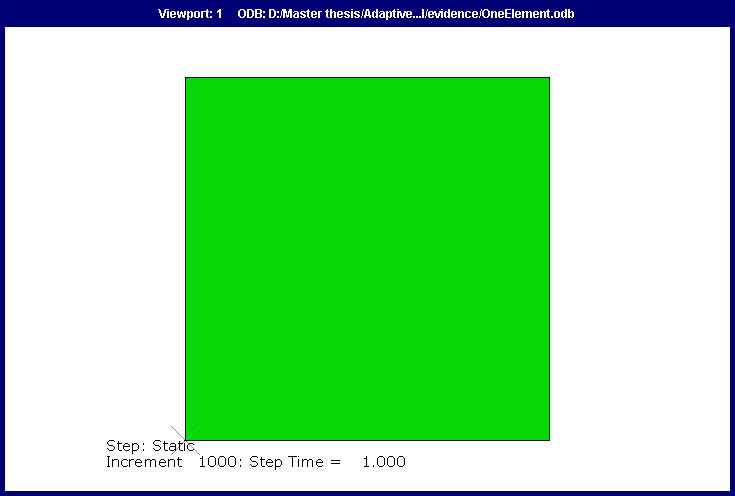
\includegraphics[width=\linewidth]{fig02a_molnar_one_element_mesh.png}\\[-0.3em]
  \small (a) Original one-element discretization
\end{minipage}\hfill
\begin{minipage}[t]{0.48\textwidth}
  \centering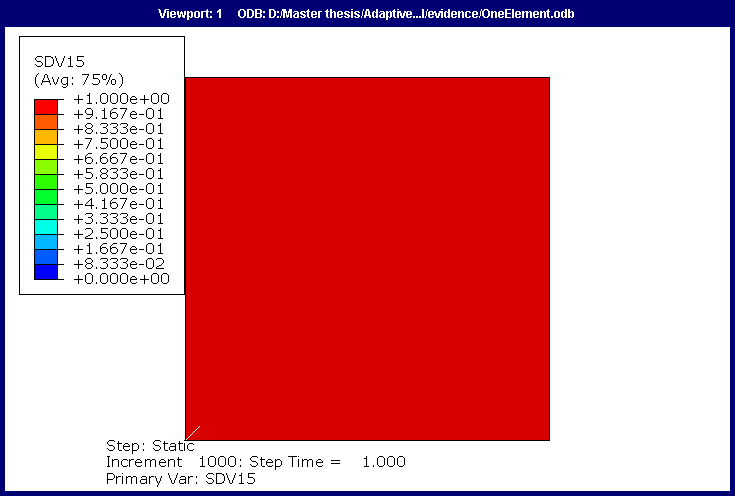
\includegraphics[width=\linewidth]{fig02a_molnar_one_element_sdv15.png}\\[-0.3em]
  \small (b) Final \texttt{SDV15}, fixed range $0\le d\le1$
\end{minipage}
\caption{Direct Abaqus CAE evidence from the unchanged Moln\'ar one-element ODB. The image establishes source execution and state evolution; it is not presented as a fracture benchmark.}
\label{fig:molnar_one_element}
\end{figure}

\section{Moln\'ar--Gravouil single-notch reproduction}
The next verification level was the author-supplied single-edge-notched specimen. Figure~\ref{fig:molnar_single_notch_mesh} shows the actual mesh reconstructed from the unchanged input deck, including the refined crack corridor, initial notch and applied boundary conditions. This calculation provides the first direct crack-evolution test of the supplied staggered UEL/UMAT implementation.

\begin{figure}[htbp]
\centering
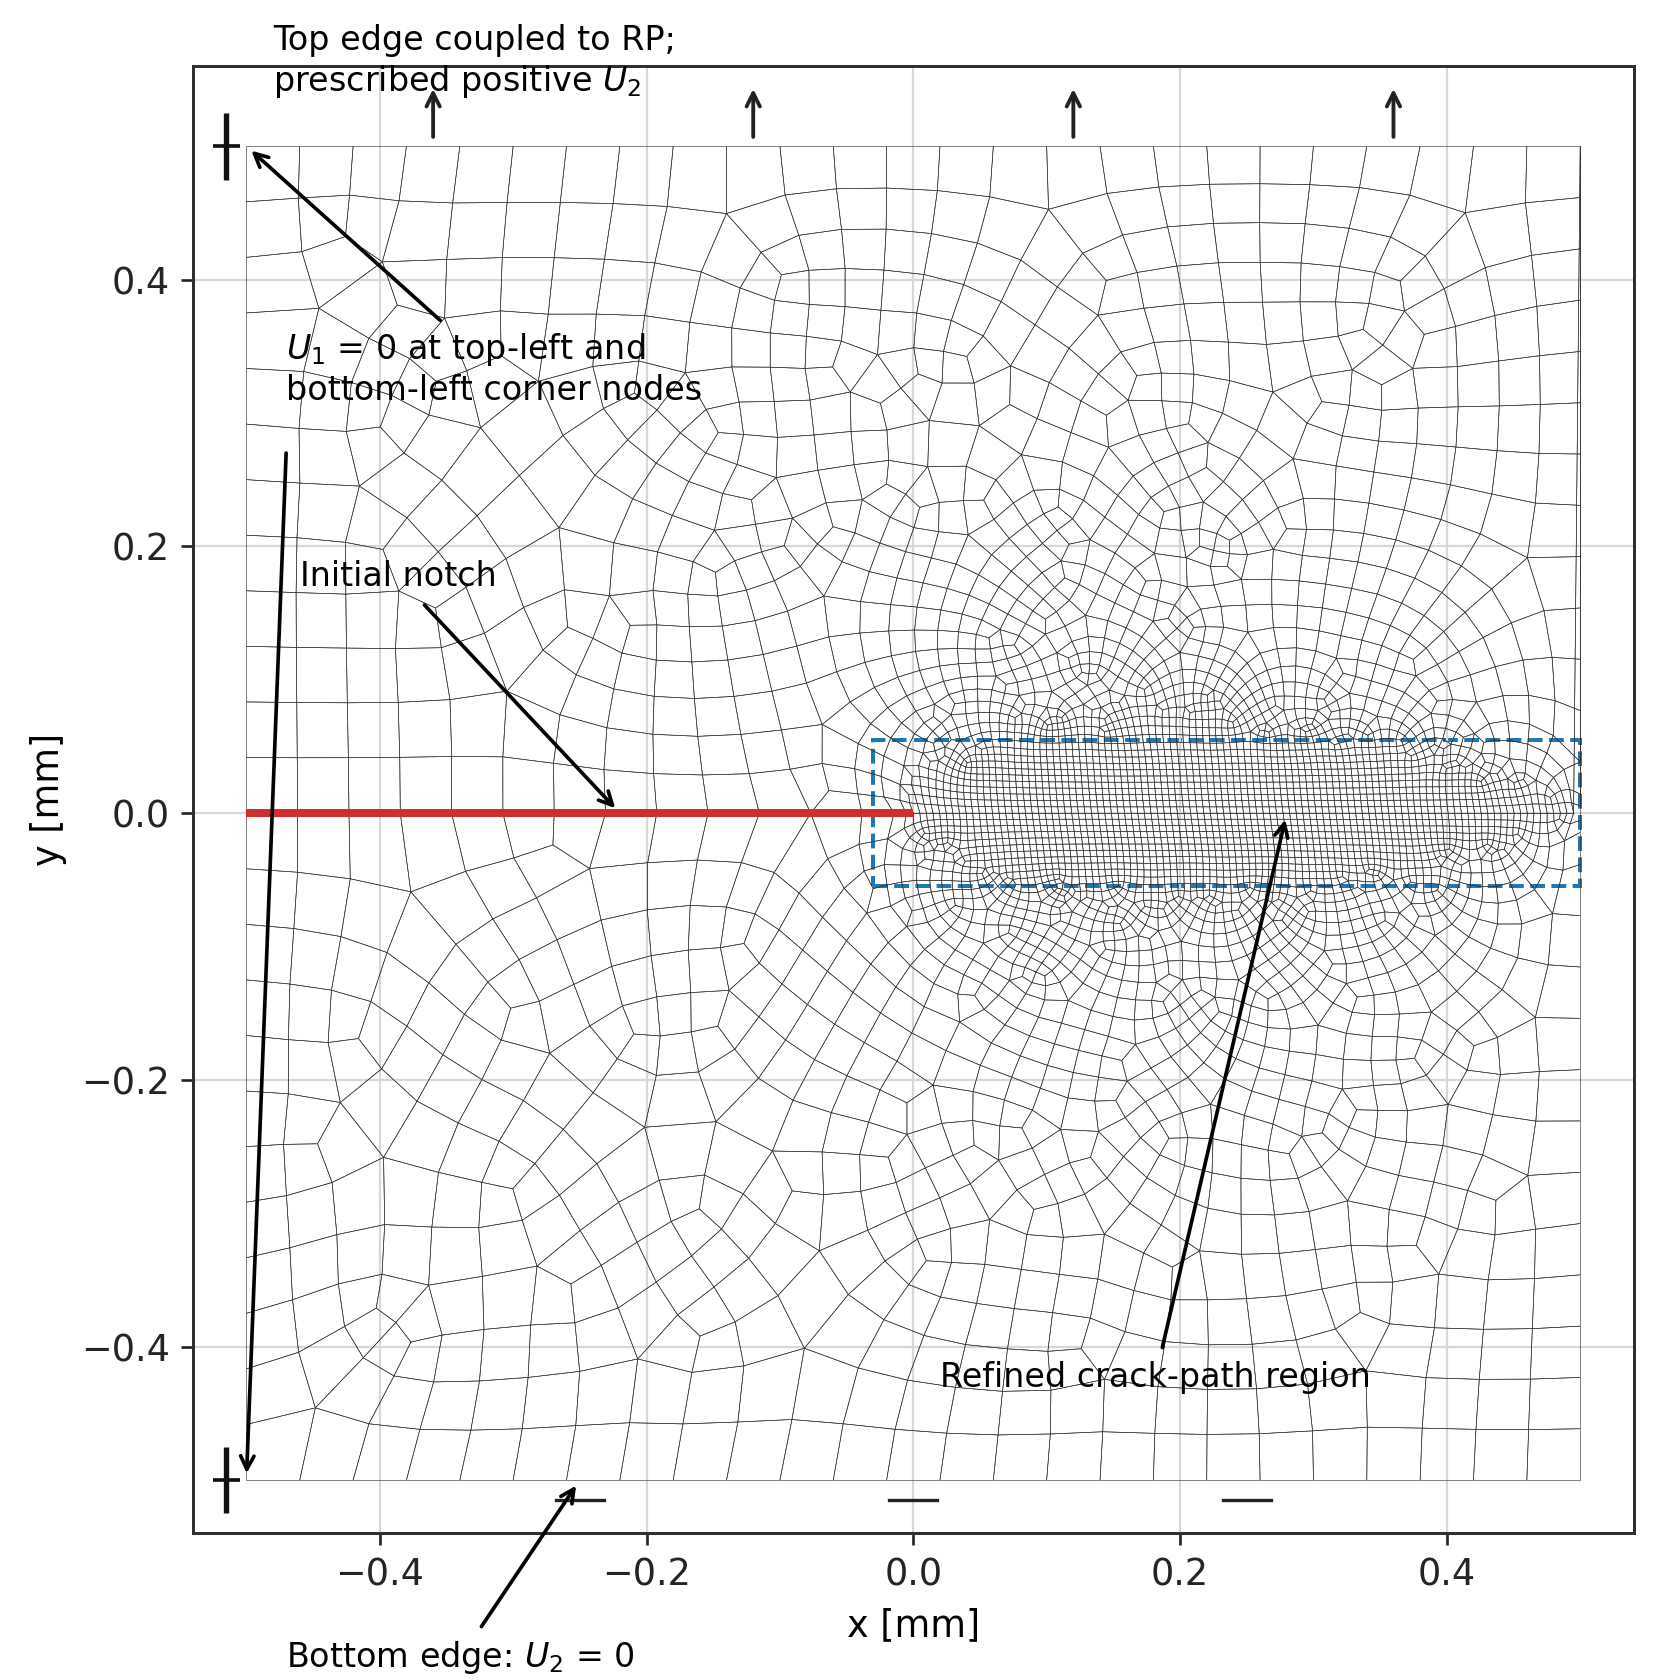
\includegraphics[width=0.78\textwidth]{fig02b_molnar_single_notch_mesh_bc.png}
\caption{Actual Moln\'ar author-supplied single-notch mesh and boundary conditions. The mesh was parsed from the unchanged input deck; no illustrative geometry was substituted.}
\label{fig:molnar_single_notch_mesh}
\end{figure}

The phase-field history in Figure~\ref{fig:molnar_phase_evolution} uses four actual converged ODB states. The displayed quantity is \texttt{SDV15}, interpreted as $d=0$ intact and $d=1$ fully damaged. The common color scale and viewport make the progression from diffuse notch-tip damage to a connected crack directly visible.

\begin{figure}[htbp]
\centering
\begin{minipage}[t]{0.24\textwidth}\centering
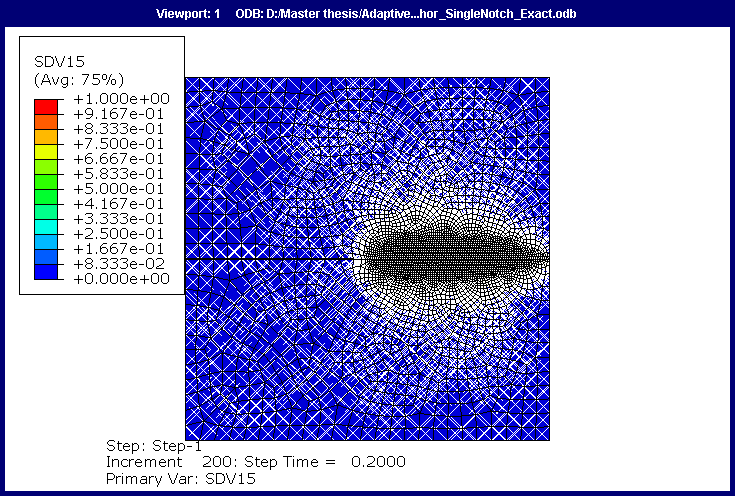
\includegraphics[width=\linewidth]{fig02c_cae_molnar_u0020.png}\\[-0.3em]\small (a) $U_2=0.0020$ mm
\end{minipage}\hfill
\begin{minipage}[t]{0.24\textwidth}\centering
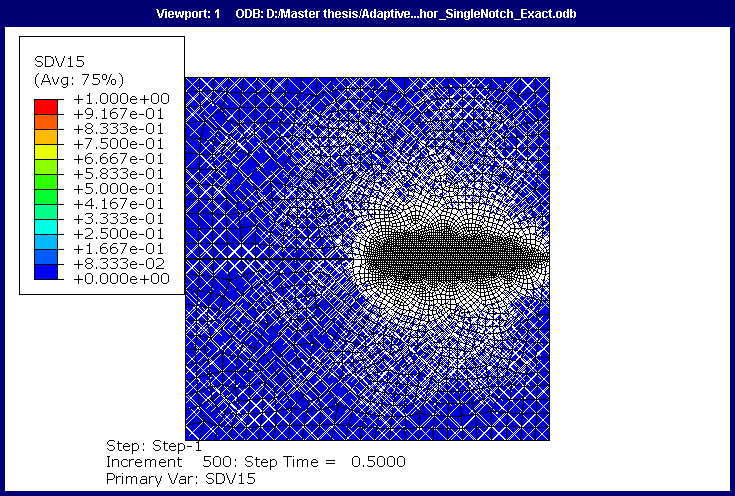
\includegraphics[width=\linewidth]{fig02c_cae_molnar_u0050.png}\\[-0.3em]\small (b) $U_2=0.0050$ mm
\end{minipage}\hfill
\begin{minipage}[t]{0.24\textwidth}\centering
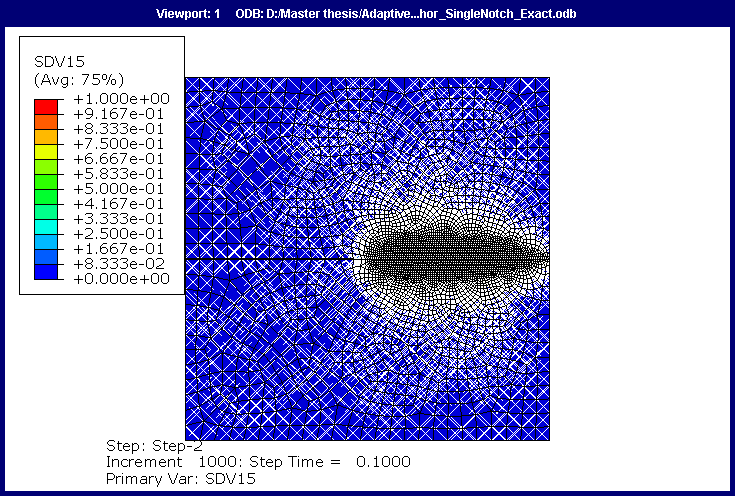
\includegraphics[width=\linewidth]{fig02c_cae_molnar_u0060.png}\\[-0.3em]\small (c) $U_2=0.0060$ mm
\end{minipage}\hfill
\begin{minipage}[t]{0.24\textwidth}\centering
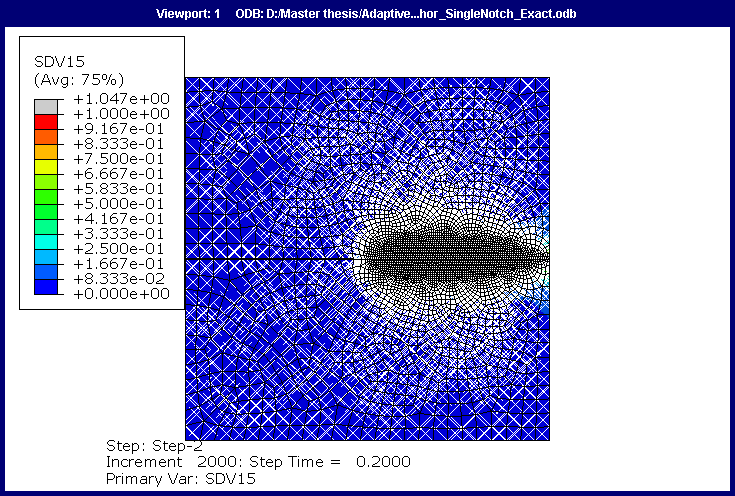
\includegraphics[width=\linewidth]{fig02c_cae_molnar_u0070.png}\\[-0.3em]\small (d) $U_2=0.0070$ mm
\end{minipage}
\caption{Direct Abaqus CAE exports of Moln\'ar single-notch \texttt{SDV15} at four converged displacement states. Every panel uses the fixed range $0\le d\le1$ and the same viewport.}
\label{fig:molnar_phase_evolution}
\end{figure}

Execution of the original supplied model did not imply exact reproduction of the published curve. The simulation peak was $0.727608\,\mathrm{kN}$ at $U_2=0.006100\,\mathrm{mm}$, while the digitized Fig.~7 reference peak was $0.690591\,\mathrm{kN}$ near $0.005584\,\mathrm{mm}$. The corresponding peak-force and peak-displacement differences were approximately $5.36\%$ and $9.25\%$, respectively. Figure~\ref{fig:molnar_rf_u} therefore reports the mismatch explicitly.

\begin{figure}[htbp]
\centering
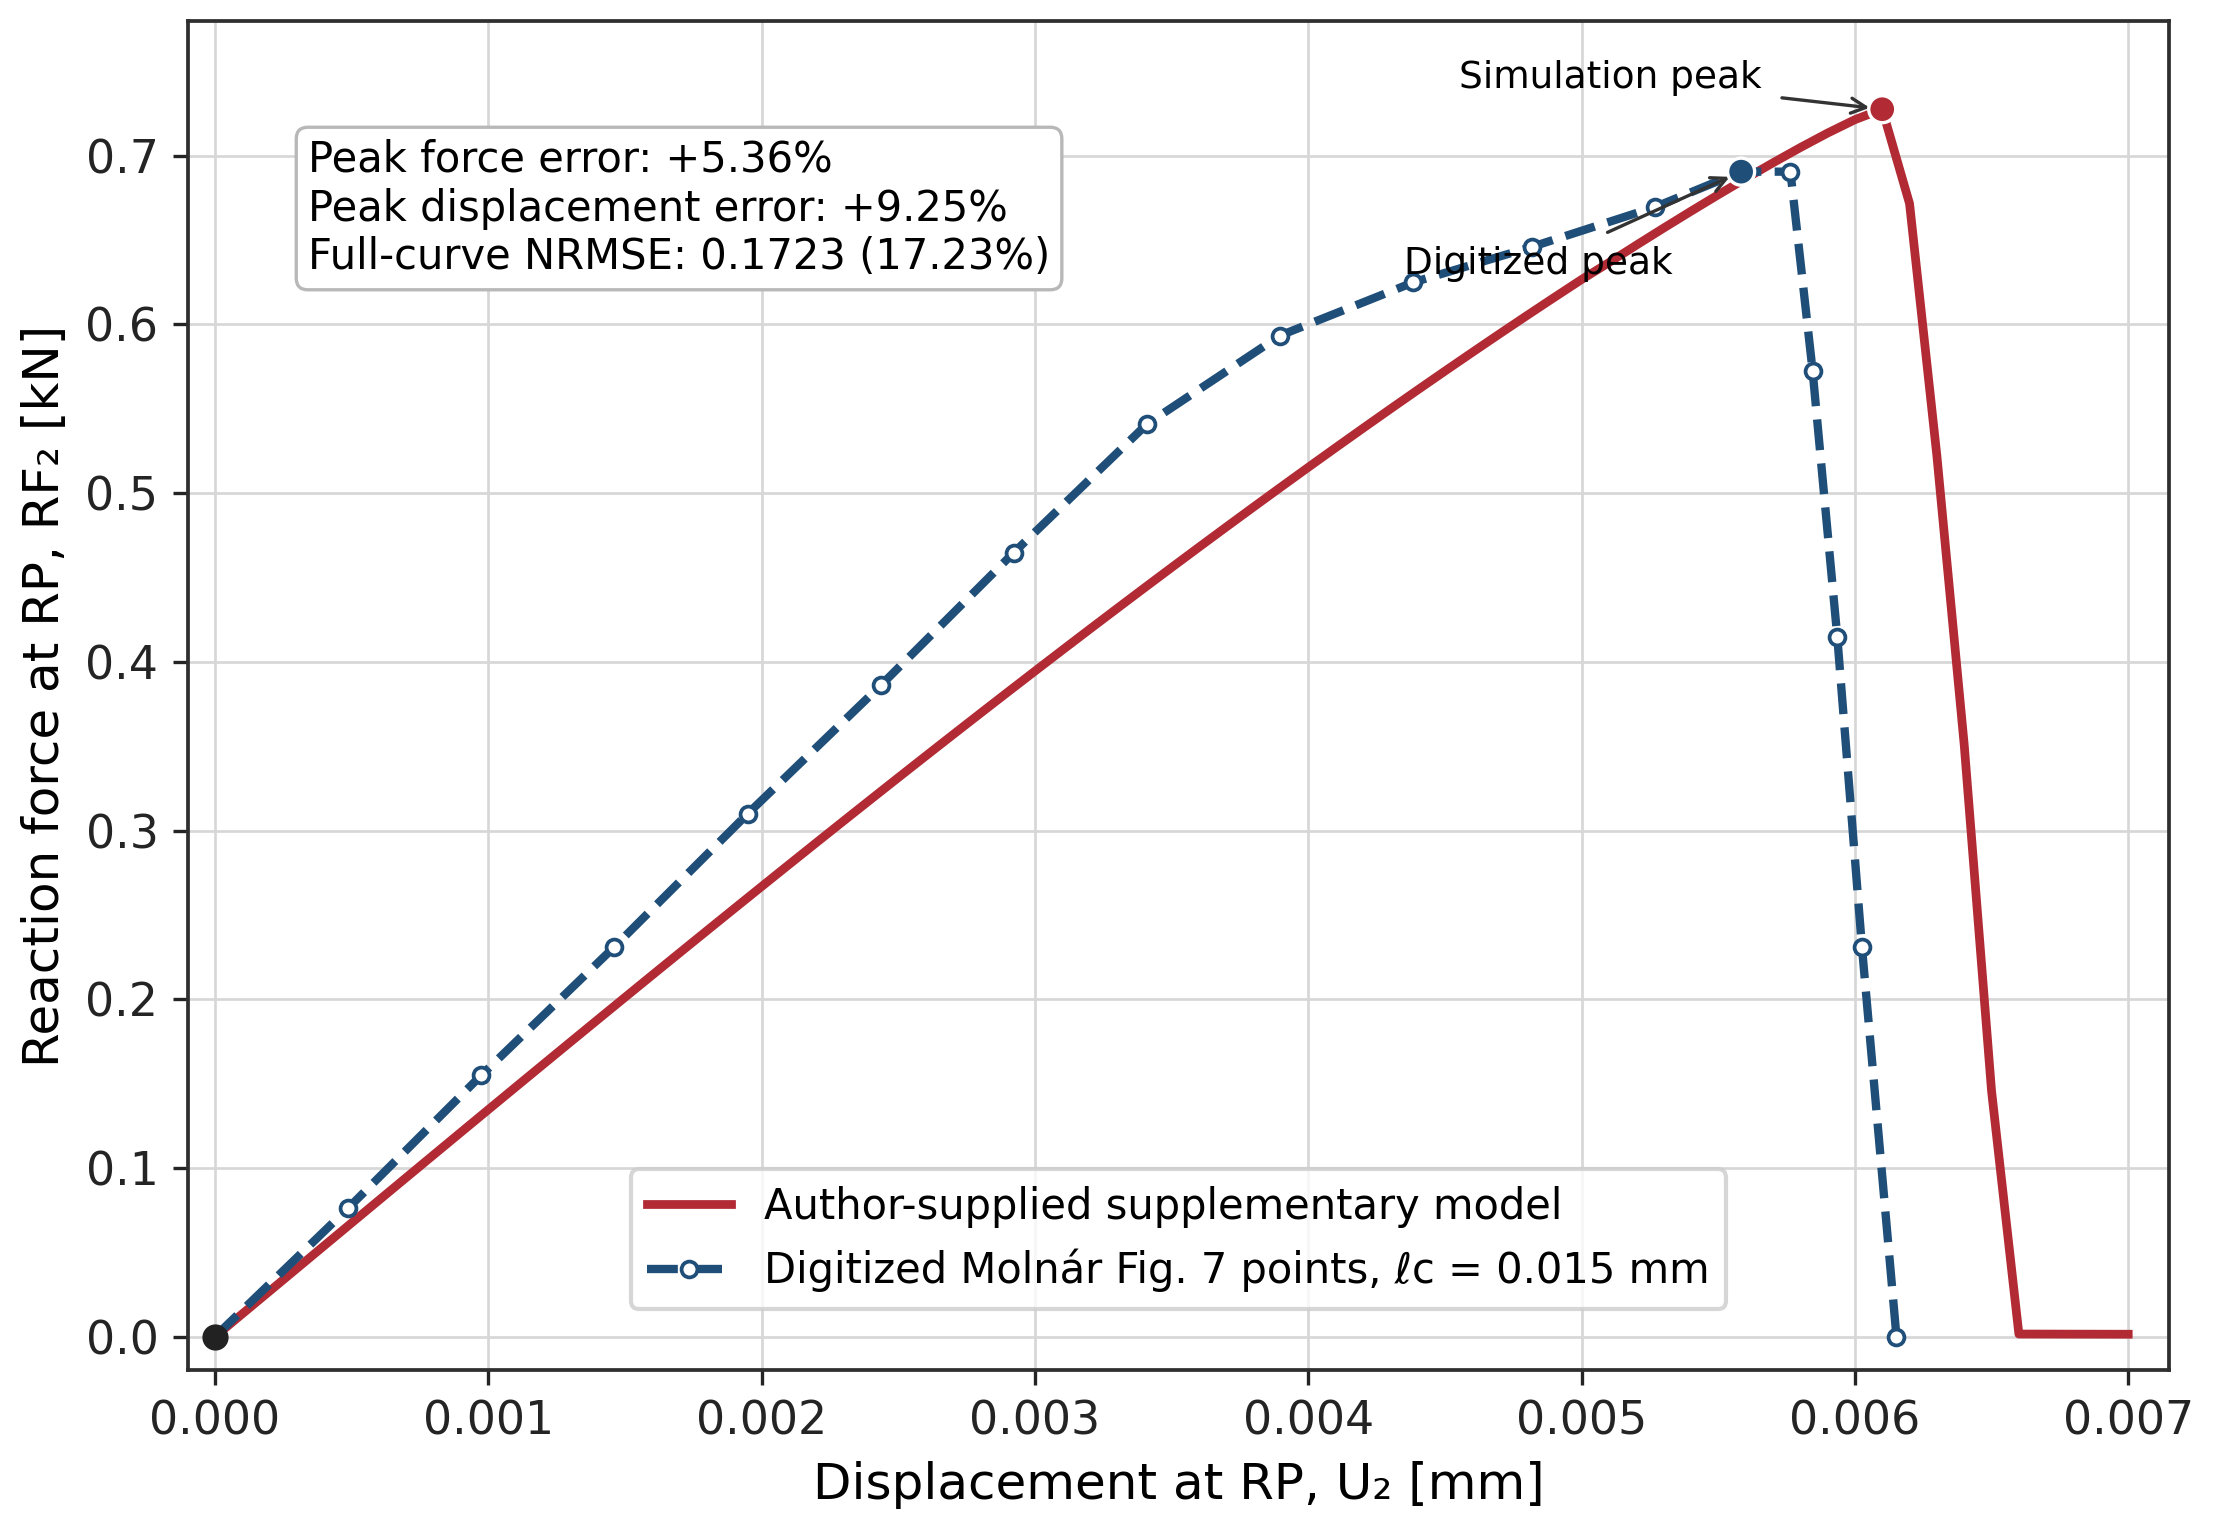
\includegraphics[width=0.76\textwidth]{fig02d_molnar_single_notch_rf_u.png}
\caption{Reaction-force--displacement comparison between the unchanged author-supplied Moln\'ar Abaqus model and the digitized $l_c=0.015\,\mathrm{mm}$ curve from Moln\'ar and Gravouil.}
\label{fig:molnar_rf_u}
\end{figure}

\section{Improved Moln\'ar Mode-I reference}
The initial discrepancy motivated a controlled mesh-resolution study rather than being hidden or treated as a remeshing effect. Figure~\ref{fig:molnar_h_convergence} summarizes the later H0/H1/H2 progression and shows how response convergence and computational cost were evaluated together. This study established the stronger fixed-mesh basis used by the subsequent refinement work.

\begin{figure}[htbp]
\centering
\begin{minipage}[t]{0.32\textwidth}\centering
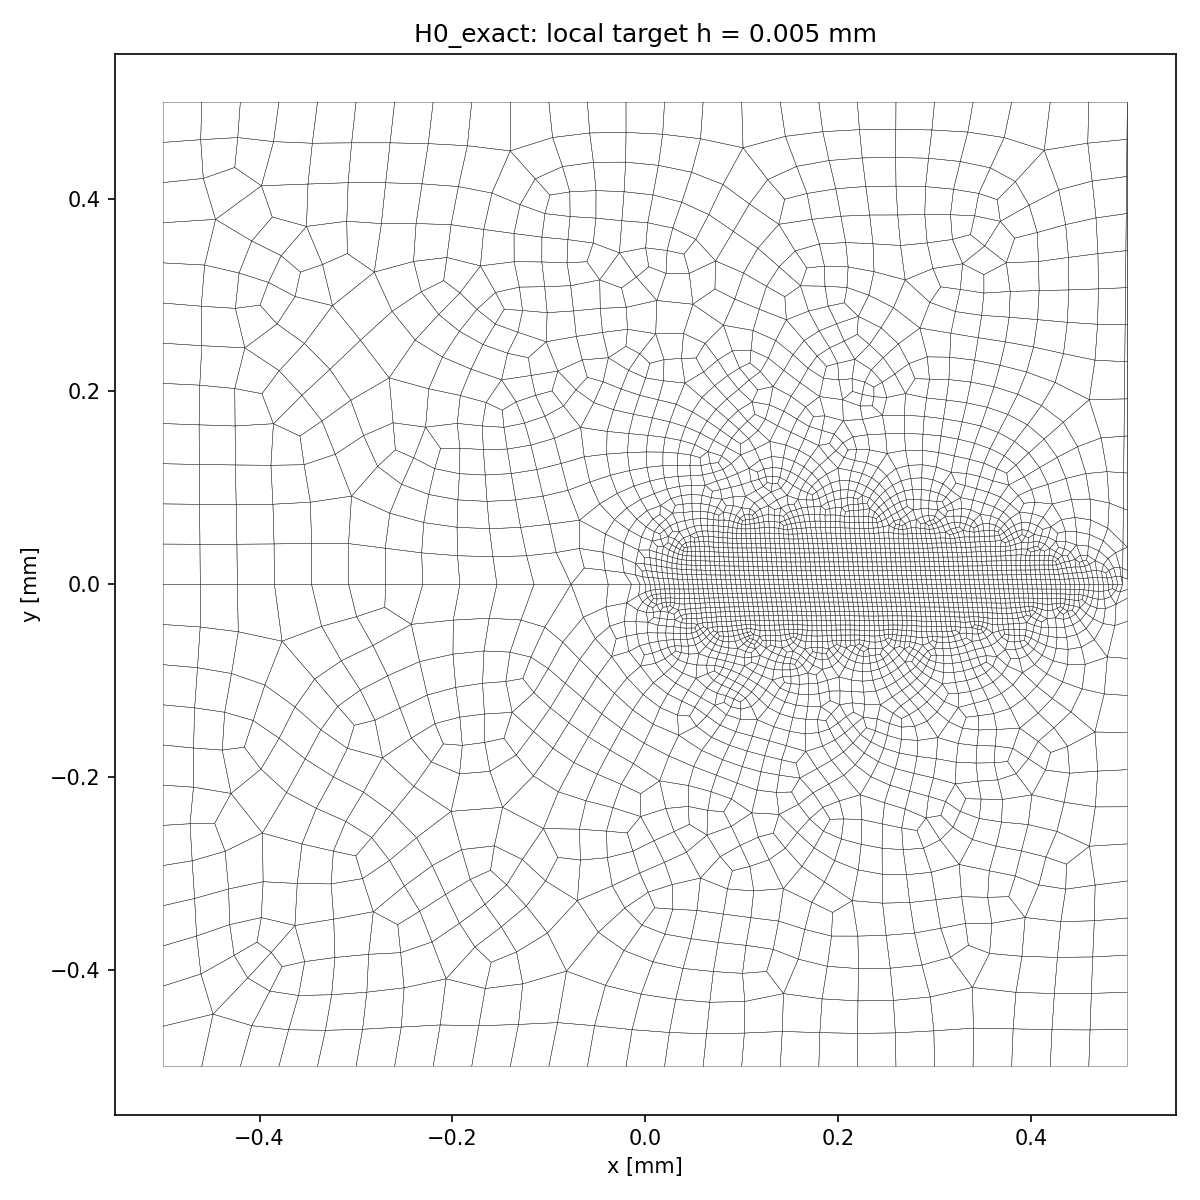
\includegraphics[width=\linewidth]{fig02f_molnar_mesh_h0.png}\\[-0.3em]\small (a) H0
\end{minipage}\hfill
\begin{minipage}[t]{0.32\textwidth}\centering
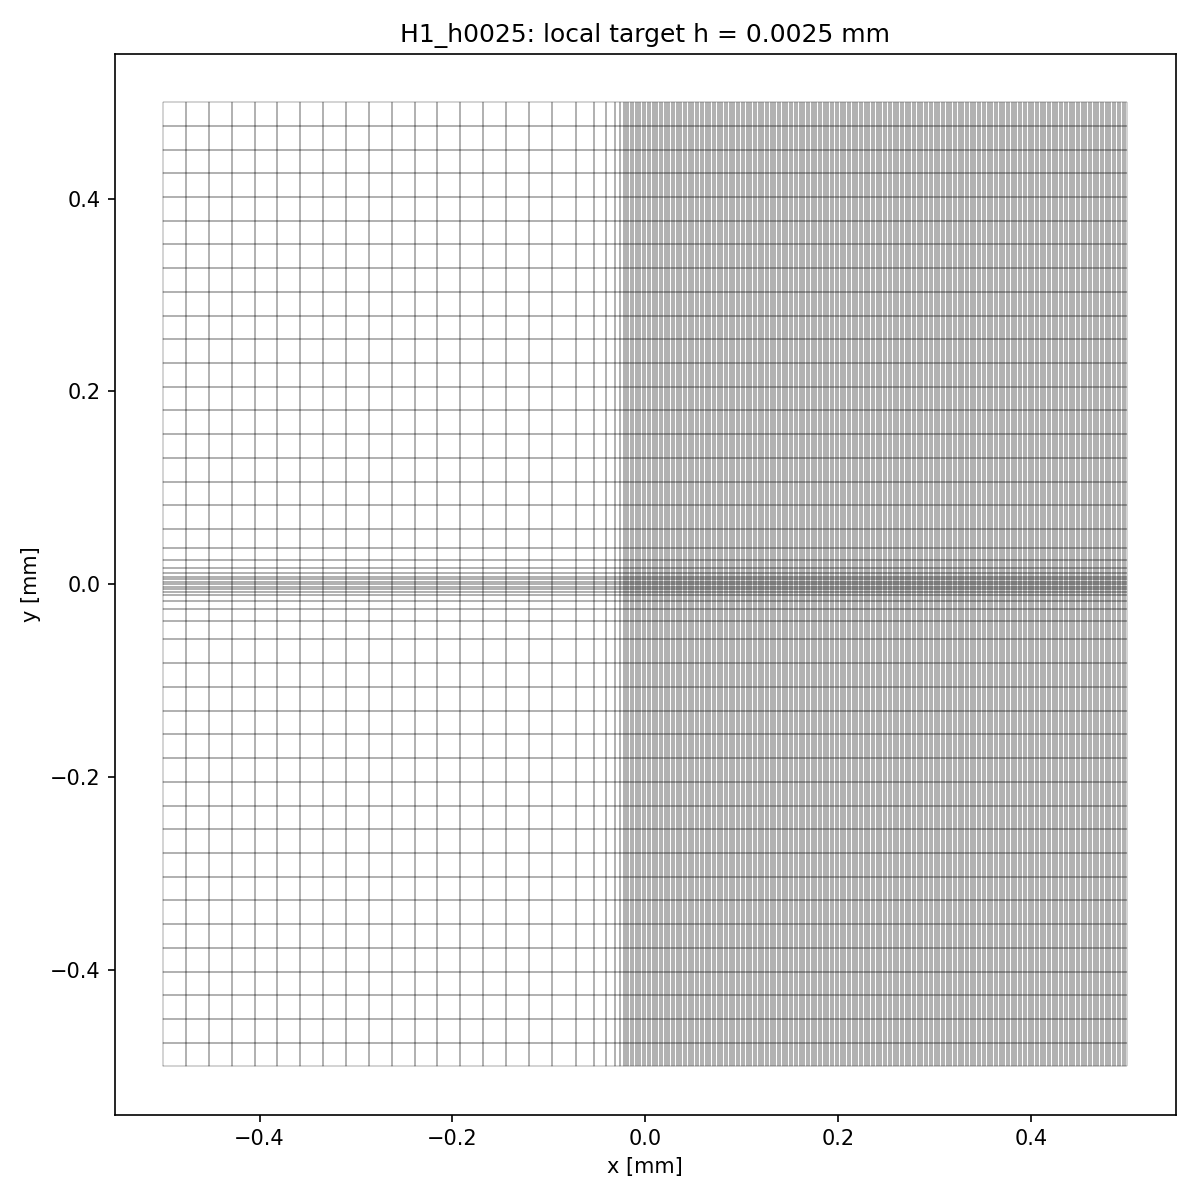
\includegraphics[width=\linewidth]{fig02f_molnar_mesh_h1.png}\\[-0.3em]\small (b) H1
\end{minipage}\hfill
\begin{minipage}[t]{0.32\textwidth}\centering
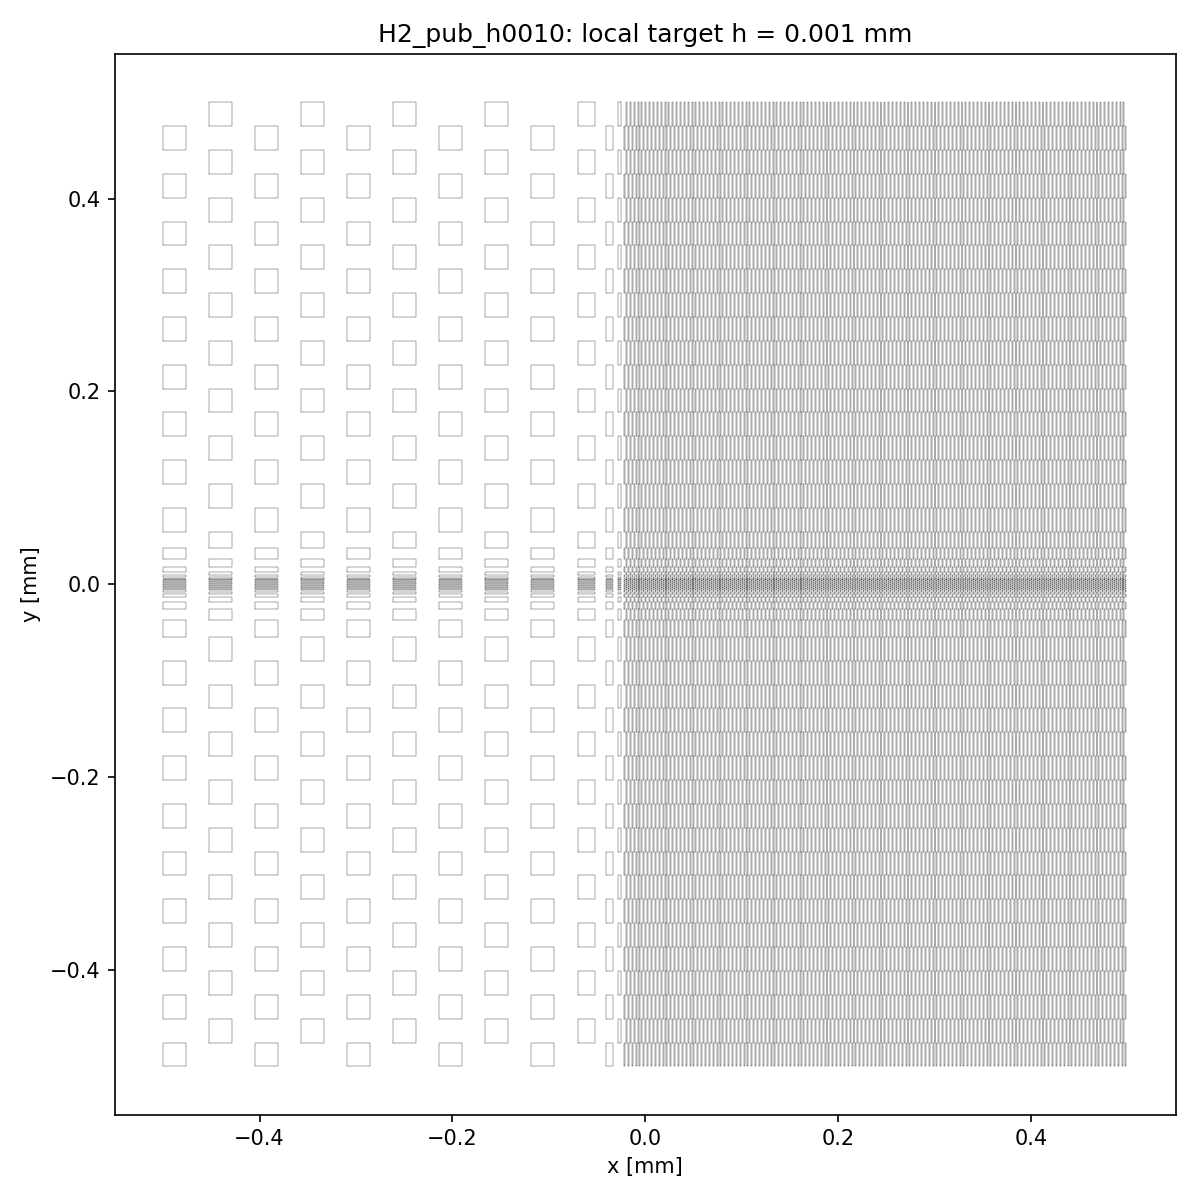
\includegraphics[width=\linewidth]{fig02f_molnar_mesh_h2.png}\\[-0.3em]\small (c) H2
\end{minipage}
\caption{Actual H0/H1/H2 Moln\'ar meshes generated by the project preprocessing chain. The panels expose the discretizations behind the convergence data in Figure~\ref{fig:molnar_h_convergence}.}
\label{fig:molnar_h_meshes}
\end{figure}

\begin{figure}[htbp]
\centering
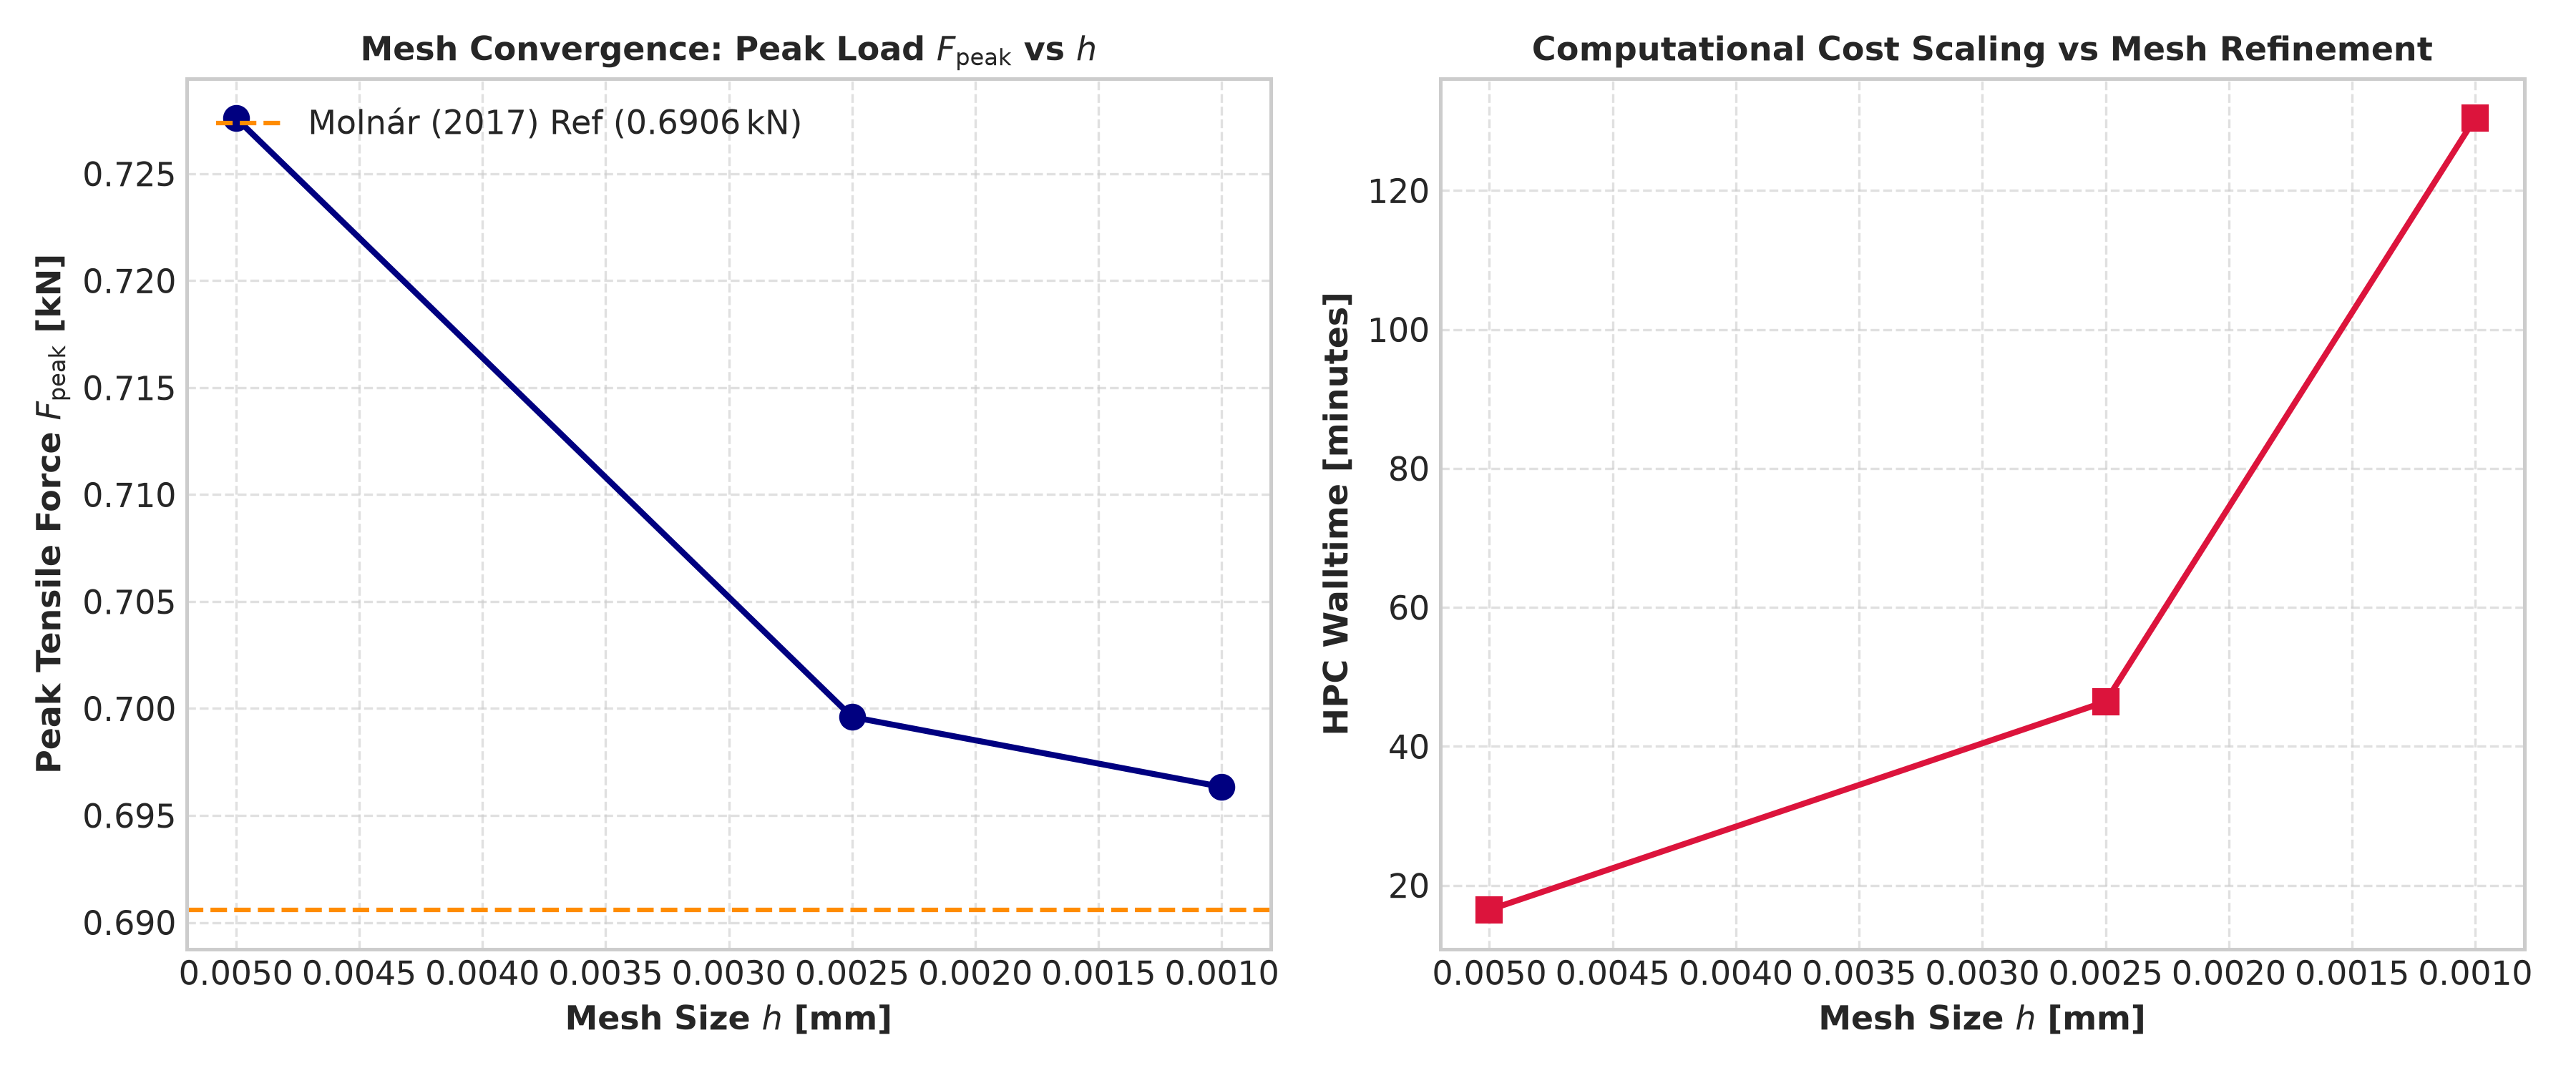
\includegraphics[width=0.92\textwidth]{fig02e_molnar_h_convergence.png}
\caption{Moln\'ar Mode-I mesh-resolution study. Response agreement is assessed together with mesh density and computational cost rather than from a single peak value.}
\label{fig:molnar_h_convergence}
\end{figure}

\section{Fixed-mesh Mode-I benchmark for the Pandey--Kumar comparison}
The benchmark is a $1\times1\,\mathrm{mm}$ square plate with a $0.5\,\mathrm{mm}$ edge crack. The material parameters are $E=210\,\mathrm{GPa}$ and $\nu=0.3$. The fracture parameters are $l_0=0.0075\,\mathrm{mm}$ and $G_c=2.7\times10^{-3}\,\mathrm{kN/mm}$. Loading is displacement controlled. In the publication, the standard phase-field calculation uses a global mesh of $0.02\,\mathrm{mm}$ and a locally refined crack corridor with $h=0.003\,\mathrm{mm}$; the displacement is applied in two steps up to $0.005\,\mathrm{mm}$ and then $0.010\,\mathrm{mm}$ \citep{Pandey2025}.

\begin{figure}[htbp]
\centering
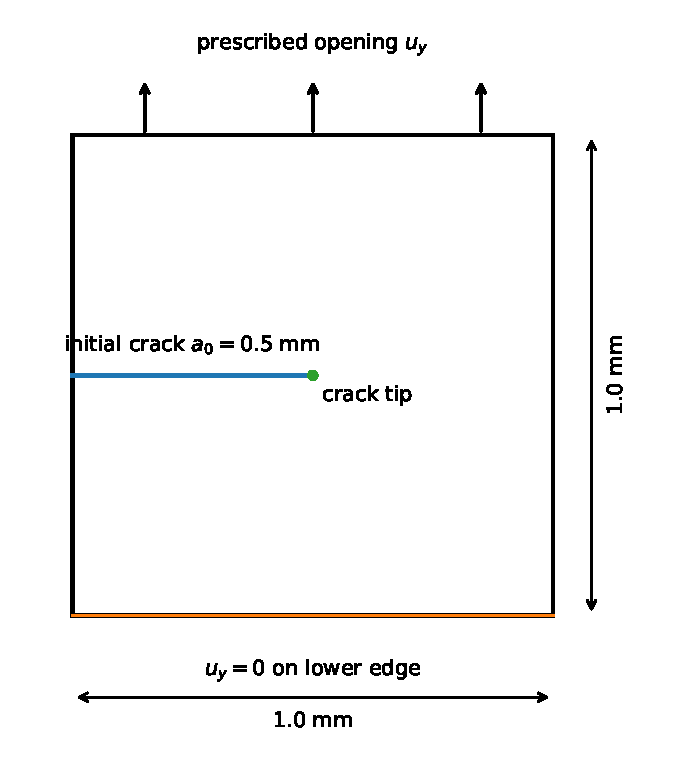
\includegraphics[width=0.62\textwidth]{fig_mode1_geometry.pdf}
\caption{Schematic of the Mode-I single-edge-crack benchmark used for the fixed-mesh reproduction and the subsequent mesh-refinement study. The crack is represented as a zero-gap discontinuity; this geometric detail is important for the elastic compliance of the specimen.}
\label{fig:mode1_geometry}
\end{figure}

\section{Fixed-mesh quantitative reproduction}
The project fixed-mesh reference calculation reached
\begin{equation}
F_{\max}=0.757778\,\mathrm{kN},\qquad u(F_{\max})=0.005857\,\mathrm{mm}.
\end{equation}
The digitized/project reference values used for the comparison are approximately $0.758\,\mathrm{kN}$ and $0.005860\,\mathrm{mm}$. Table~\ref{tab:baseline_comparison} summarizes the scalar comparison.

\begin{table}[htbp]
\centering
\caption{Fixed-mesh Mode-I reproduction compared with the project reference values extracted from the published benchmark.}
\label{tab:baseline_comparison}
\begin{tabular}{lccc}
\toprule
Quantity & Reference & Reproduction & Relative difference \\
\midrule
Peak force $F_{\max}$ & $0.758000\,\mathrm{kN}$ & $0.757778\,\mathrm{kN}$ & $-0.029\%$ \\
Displacement at peak & $0.005860\,\mathrm{mm}$ & $0.005857\,\mathrm{mm}$ & $-0.051\%$ \\
\bottomrule
\end{tabular}
\end{table}

The complete force--displacement curve remains the preferred comparison quantity. The peak values are reported here because they provide a compact check that the reconstructed benchmark has the correct force scale and localization displacement before changing the mesh-generation procedure.

The accepted standard ODB also contains the matched-state fields required for a final standard-versus-adaptive comparison. That combined figure is deferred until the adaptive calculation provides verified terminal states at matching displacements.

\section{Geometry sanity check for later adaptive models}
The baseline was also used as a model-level diagnostic. A later refinement attempt accidentally represented the pre-crack as a finite-width rectangular slot. Its initial stiffness was $75.47\,\mathrm{kN/mm}$, whereas the accepted fixed-mesh baseline was about $138.15\,\mathrm{kN/mm}$. Replacing the slot by a zero-gap seam restored the pre-analysis stiffness to $141.82\,\mathrm{kN/mm}$, a difference of about $+2.65\%$ from the baseline. This comparison identified a geometry error before interpreting the discrepancy as a phase-field or remeshing effect.

\section{Baseline conclusion}
The fixed-mesh Mode-I response is sufficiently well reproduced to serve as the current reference for the refined calculation. The later comparison therefore considers the complete force--displacement curve, peak force, displacement at peak, crack path and computational cost. Agreement of a single scalar quantity is not by itself considered sufficient validation.

\chapter{Abaqus-Native Error-Guided Mesh Refinement}
\label{ch:refinement}

\section{Role of \texttt{MISESERI}}
Abaqus provides recovered-stress error indicators for standard continuum elements. In the present workflow, the companion UMAT elements reproduce the mechanical fields of the user-element discretization so that Abaqus can evaluate \texttt{MISESERI}. The indicator measures stress-discretization error associated with the recovered von Mises stress field; it is not a measure of phase-field discretization error. Its role is therefore predictive: it identifies mechanically under-resolved regions in the preliminary solution that are plausible candidates for subsequent fracture localization.

\begin{figure}[htbp]
\centering
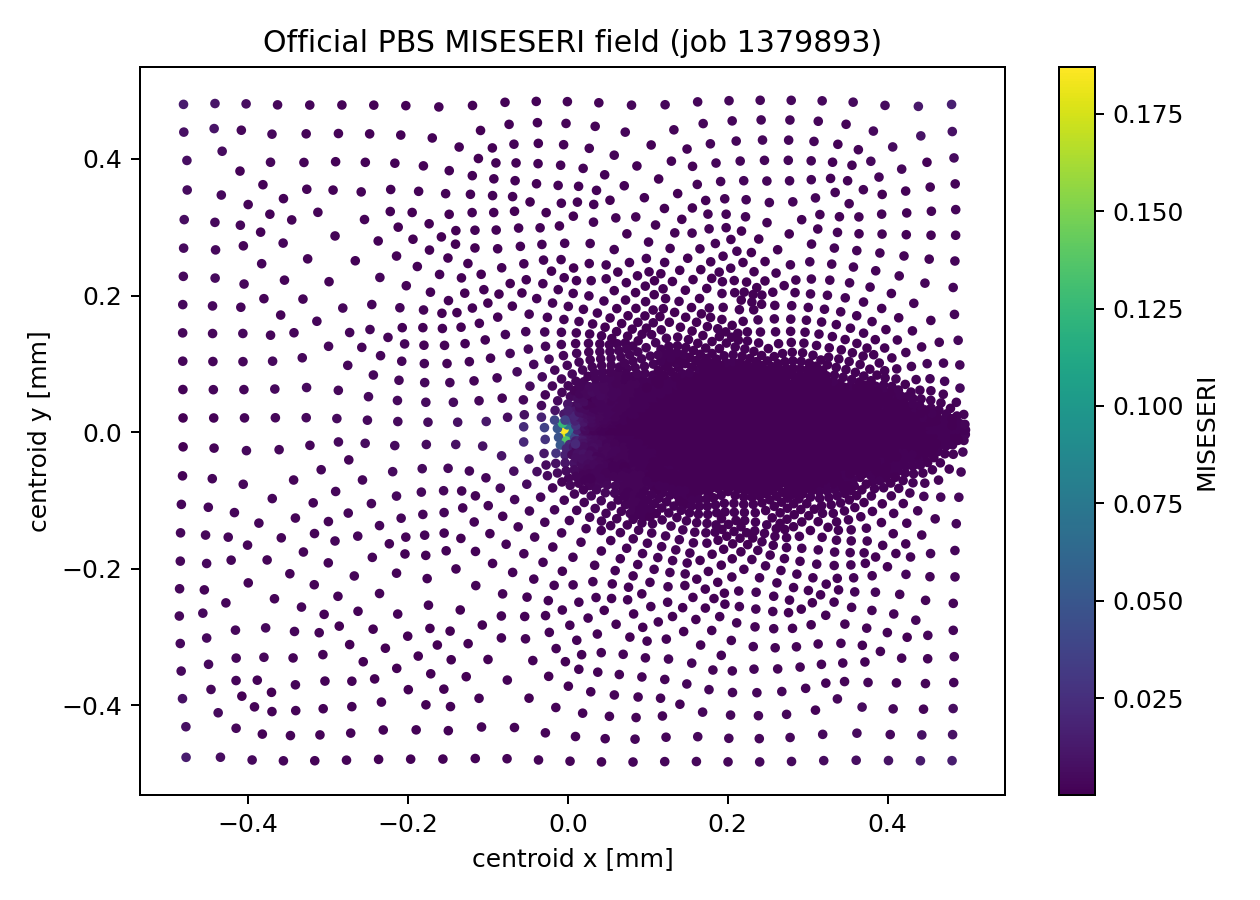
\includegraphics[width=0.82\textwidth]{fig04_miseseri_spatial_map.png}
\caption{Spatial distribution of the official PBS-extracted \texttt{MISESERI} field from coarse pre-analysis job \texttt{1379893.mmaster02}. The plot is generated from the 3,930-row extraction CSV with SHA-256 \texttt{49b0c5f7a784f361...}; the ODB, CSV and repaired validation are recorded together in the Stage-F4 replacement evidence. This is a derived plot of Abaqus element-field output, not a reconstructed phase-field contour.}
\label{fig:miseseri_spatial_map}
\end{figure}

\section{Reference-faithful two-job workflow}
The implemented Python sequence follows the structure reported by Pandey and Kumar \citep{Pandey2025}:
\begin{enumerate}
  \item create the coarse physical model and the coincident output/facsimile layer;
  \item run the preliminary analysis and request \texttt{MISESERI}, \texttt{MISESAVG}, stress, volume, reaction force and displacement;
  \item define an Abaqus \texttt{RemeshingRule} on the assembly set corresponding to \texttt{All\_elem};
  \item open the preliminary ODB and execute \texttt{model.adaptiveRemesh(odb=odb)};
  \item export the newly refined physical mesh;
  \item reconstruct the phase-field UEL layer, mechanical UEL layer and visualization/UMAT layer on the new connectivity;
  \item audit node coordinates, element connectivity, sets, boundary conditions, element types and property assignments before the fracture solve.
\end{enumerate}

\begin{figure}[htbp]
\centering
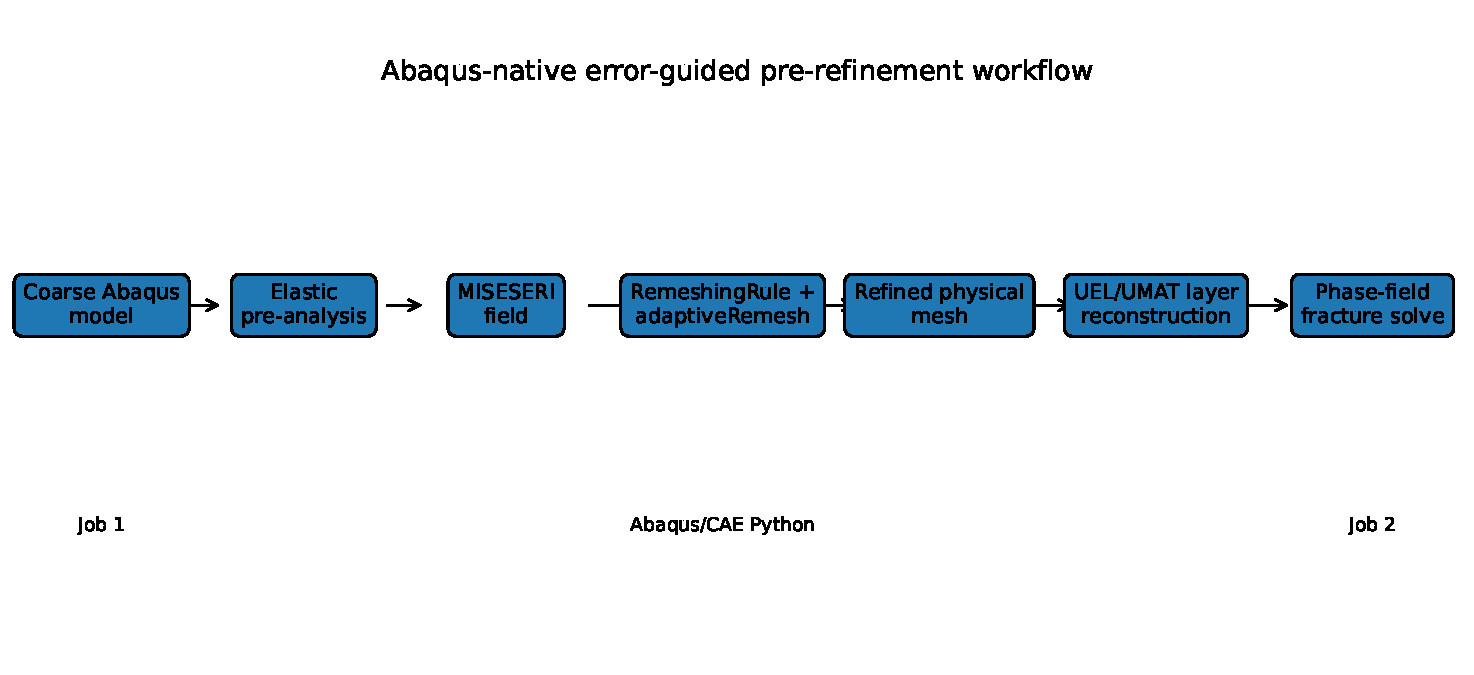
\includegraphics[width=0.98\textwidth]{fig_refinement_workflow.pdf}
\caption{Computational sequence used to reproduce the Pandey--Kumar error-guided pre-refinement method. The fracture calculation begins from a virgin state on the final refined mesh; state transfer is not part of this two-job pre-refinement workflow.}
\label{fig:refinement_workflow}
\end{figure}

A headless qualification revealed an important Abaqus scripting detail. The operation \texttt{adaptiveRemesh} already modifies the model mesh. Calling \texttt{generateMesh()} afterwards reapplied the original part seeds and overwrote the refined mesh. Removing that second meshing call changed the test problem from an unchanged $553$-element mesh to a genuinely refined $2{,}222$-element mesh. This check was added as a regression condition: an adaptive-remesh operation that leaves topology unchanged when nontrivial \texttt{MISESERI} requires refinement is treated as a failed qualification.

\section{Mode-I reference settings}
For the principal Mode-I case, Pandey and Kumar report a global element size of $0.02\,\mathrm{mm}$ and a local element size of $0.001\,\mathrm{mm}$ \citep{Pandey2025}. The remeshing rule uses \texttt{errorTarget=1.0} and \texttt{refinementFactor=10}, with coarsening disabled. Their refined Mode-I mesh contains $13{,}941$ triangular and quadrilateral elements. The present reconstruction uses these nominal settings together with the corrected sharp seam.

Figure~\ref{fig:coarse_adaptive_meshes} provides direct CAE mesh evidence for the two ends of the implemented workflow. The sensitivity cases remain represented by their audited counts until their distinct mesh artifacts can be exported with the same viewport; no reconstructed pattern is substituted.

\begin{figure}[htbp]
\centering
\begin{minipage}[t]{0.48\textwidth}\centering
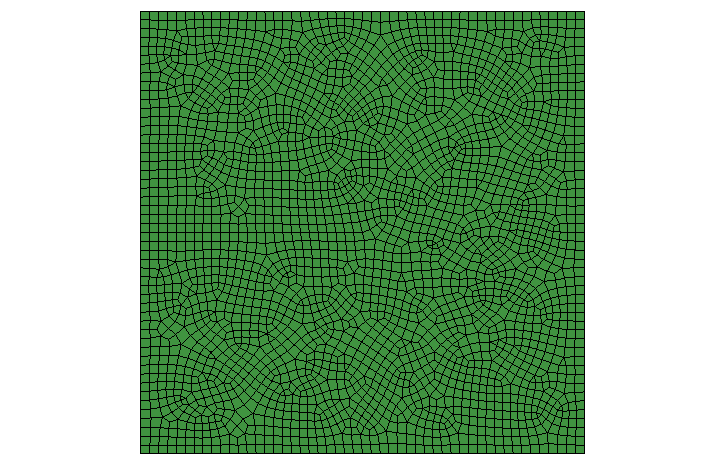
\includegraphics[width=\linewidth]{fig03a_coarse_mesh_cae.png}\\[-0.3em]\small (a) Coarse pre-analysis mesh
\end{minipage}\hfill
\begin{minipage}[t]{0.48\textwidth}\centering
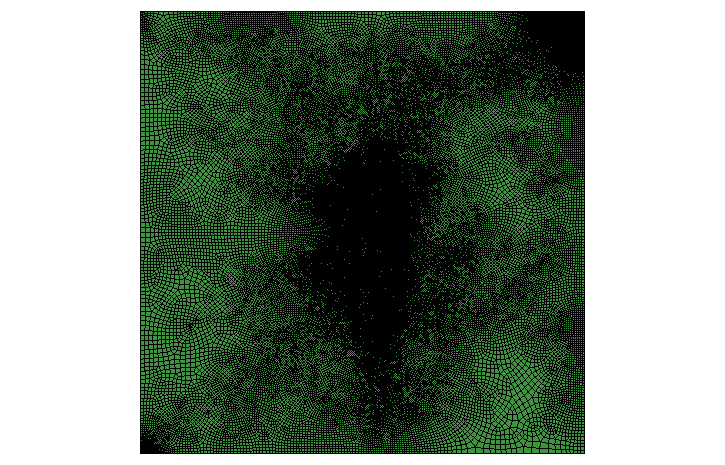
\includegraphics[width=\linewidth]{fig13_adaptive_71320_mesh_cae.png}\\[-0.3em]\small (b) Nominal $1\%$ refined physical mesh
\end{minipage}
\caption{Direct Abaqus CAE mesh exports from the coarse pre-analysis input and the accepted nominal refined physical input. The dense central corridor in (b) is the actual native-remeshing result, not an illustrative reconstruction.}
\label{fig:coarse_adaptive_meshes}
\end{figure}

\section{Observed mesh-density discrepancy}
The reconstructed $1\%$ case produced $71{,}320$ physical elements, substantially more than the published $13{,}941$. Because a model may solve correctly while still failing to reproduce the reference refinement pattern, a separate preprocessing sensitivity study was performed without changing the fracture parameters. For the current reconstruction, $2\%$ and $5\%$ error targets generated $15{,}396$ and $4{,}194$ elements, respectively.

\begin{figure}[htbp]
\centering
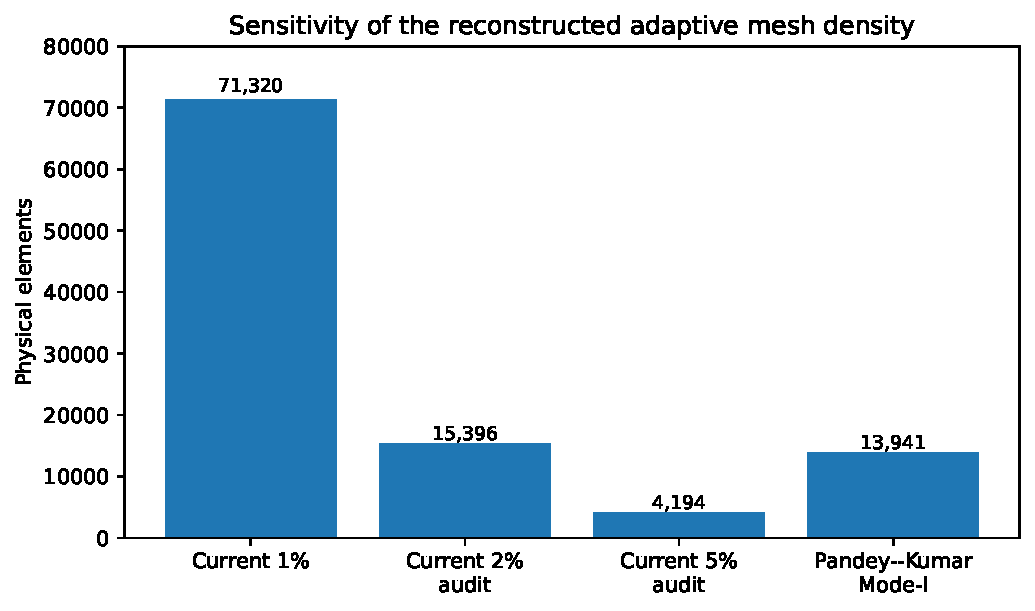
\includegraphics[width=0.82\textwidth]{fig_adaptivity_element_counts.pdf}
\caption{Physical-element counts obtained from the present Abaqus-native refinement reconstruction. The $2\%$ and $5\%$ cases are sensitivity calculations, not replacements for the nominal $1\%$ production setting. The publication reports $13{,}941$ elements for its Mode-I proposed mesh.}
\label{fig:adaptive_counts}
\end{figure}

The sensitivity study demonstrates that the remeshing outcome is highly sensitive to the interpretation of the error target and the resulting Abaqus sizing field. It does \emph{not} establish that the publication used $2\%$ in the Mode-I result. In fact, the paper explicitly lists \texttt{errorTarget=1.0} in its remeshing-rule function and separately reports a later sensitivity study with other error-target values. The origin of the remaining element-count discrepancy must therefore be stated as unresolved. Plausible contributors to examine include the precise pre-analysis loading history, the spatial region attached to the remeshing rule, Abaqus release-dependent sizing behaviour, and details of the coarse-mesh topology that are not completely recoverable from the publication.

\section{Interpretation}
Task 4 is considered implemented at the level of the execution chain: Abaqus-native refinement runs headlessly, produces a genuinely changed mesh, and the result can be converted into the layered UEL/UMAT model with deterministic connectivity checks. Task 5 remains a quantitative reproduction problem because the refined mesh density and the final fracture response must both be compared with the publication. The current $1\%$ fracture calculation is discussed in Chapter~\ref{ch:production} and is still running at the time of report preparation.

\chapter{Nonmatching State Transfer and Restart}
\label{ch:transfer}

\section{Why state transfer is required}
Pre-refinement does not require state transfer because the final fracture calculation starts from the virgin state. Evolving remeshing is different: when the mesh changes after damage has developed, the receiving discretization must recover the mechanical displacement, phase field and irreversible history state of the donor analysis. A technically valid interpolation is not sufficient; the restarted model must also remain mechanically and thermodynamically consistent.

\section{Transferred quantities and mapping spaces}
The implemented transfer path distinguishes nodal and integration-point quantities. Displacement and phase field are transferred in nodal space using donor-element search and isoparametric interpolation. The crack-driving history field is stored at integration points and is therefore transferred with a separate Gauss-point mapping procedure. Crack flanks are treated as separate topological regions to avoid interpolation across an existing slit.

The receiving state is checked for phase bounds and history positivity. For irreversible fracture, preservation of the donor history is more important than reproducing a visually smooth field because a reduced history value can permit unphysical damage recovery.

\section{Runtime state ingestion}
An early transfer attempt generated a mapping artifact correctly but did not alter the running solution because the active UEL initialization path did not consume the prepared state. This distinction led to a redesign in which the transfer data are loaded explicitly at runtime through \texttt{UEXTERNALDB} and shared with the user-element routines. Subsequent tests confirmed that the transferred displacement, phase and history data were actually installed into the receiver analysis.

Figure~\ref{fig:transfer_phase_history} shows the actual checkpoint phase and history fields used by the transfer workflow. It complements the numerical transfer tables by making the donor localization state visible.

\begin{figure}[htbp]
\centering
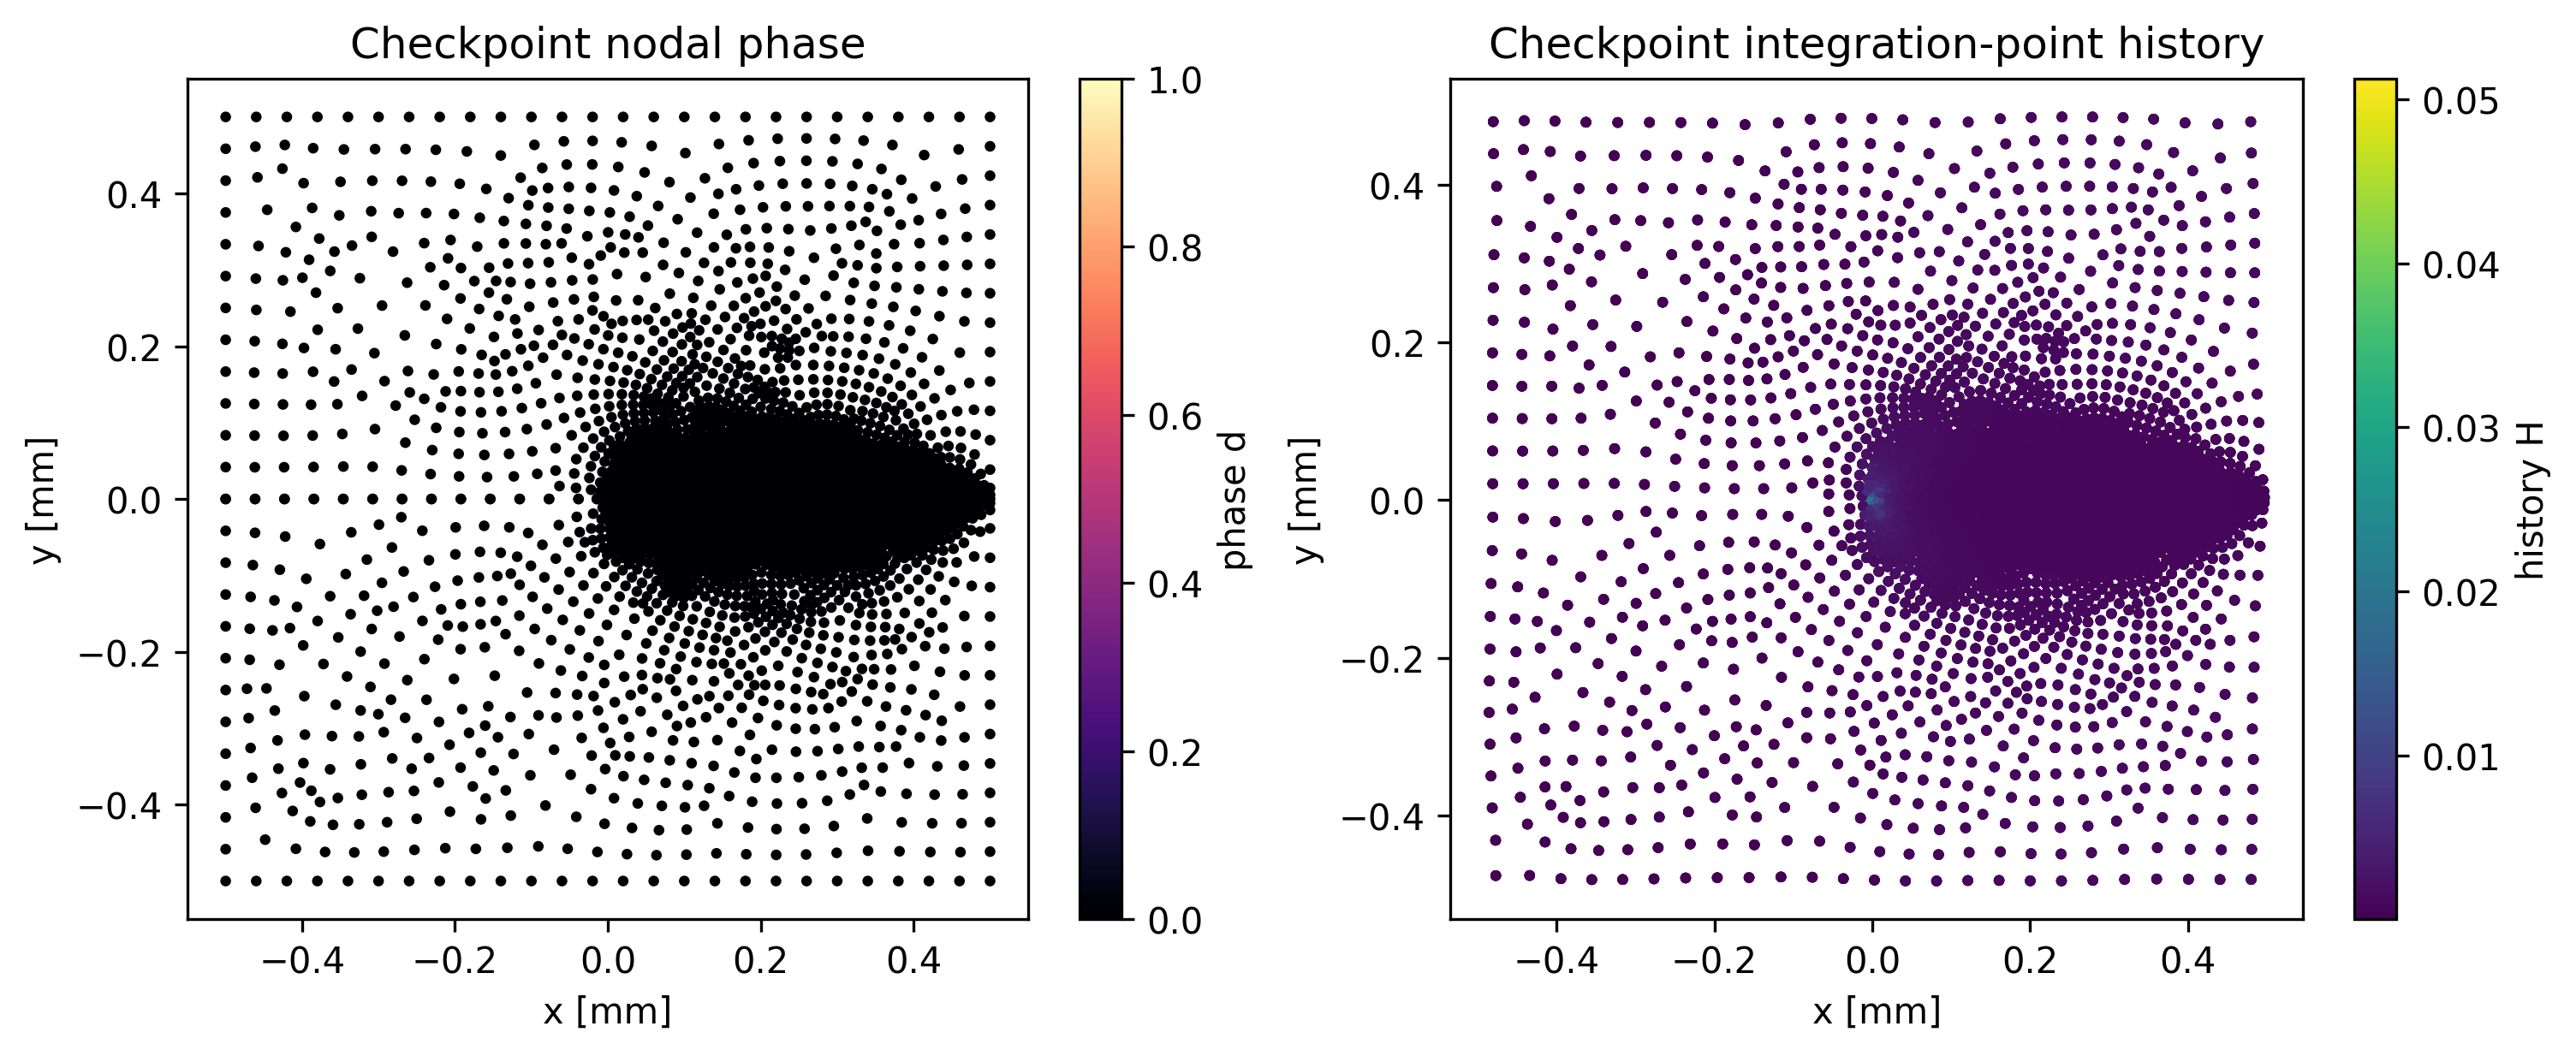
\includegraphics[width=0.94\textwidth]{fig07_state_transfer_phase_history.png}
\caption{Checkpoint phase-field and history-field evidence used by the nonmatching state-transfer workflow. The panels originate from extracted simulation fields at the same donor checkpoint.}
\label{fig:transfer_phase_history}
\end{figure}

\section{Restart sequence}
To separate state installation from subsequent equilibration, the receiver calculation is divided conceptually into four stages:
\begin{enumerate}
  \item install the transferred state and prescribed donor kinematics;
  \item establish mechanical equilibrium while the phase field is held fixed;
  \item release the phase-field constraints and allow the coupled state to relax;
  \item continue the external loading.
\end{enumerate}
This sequence improved numerical robustness, but it must not be interpreted as a guarantee of physical continuity. The decisive comparison is the state after the phase field has been released and relaxed.

\begin{figure}[htbp]
\centering
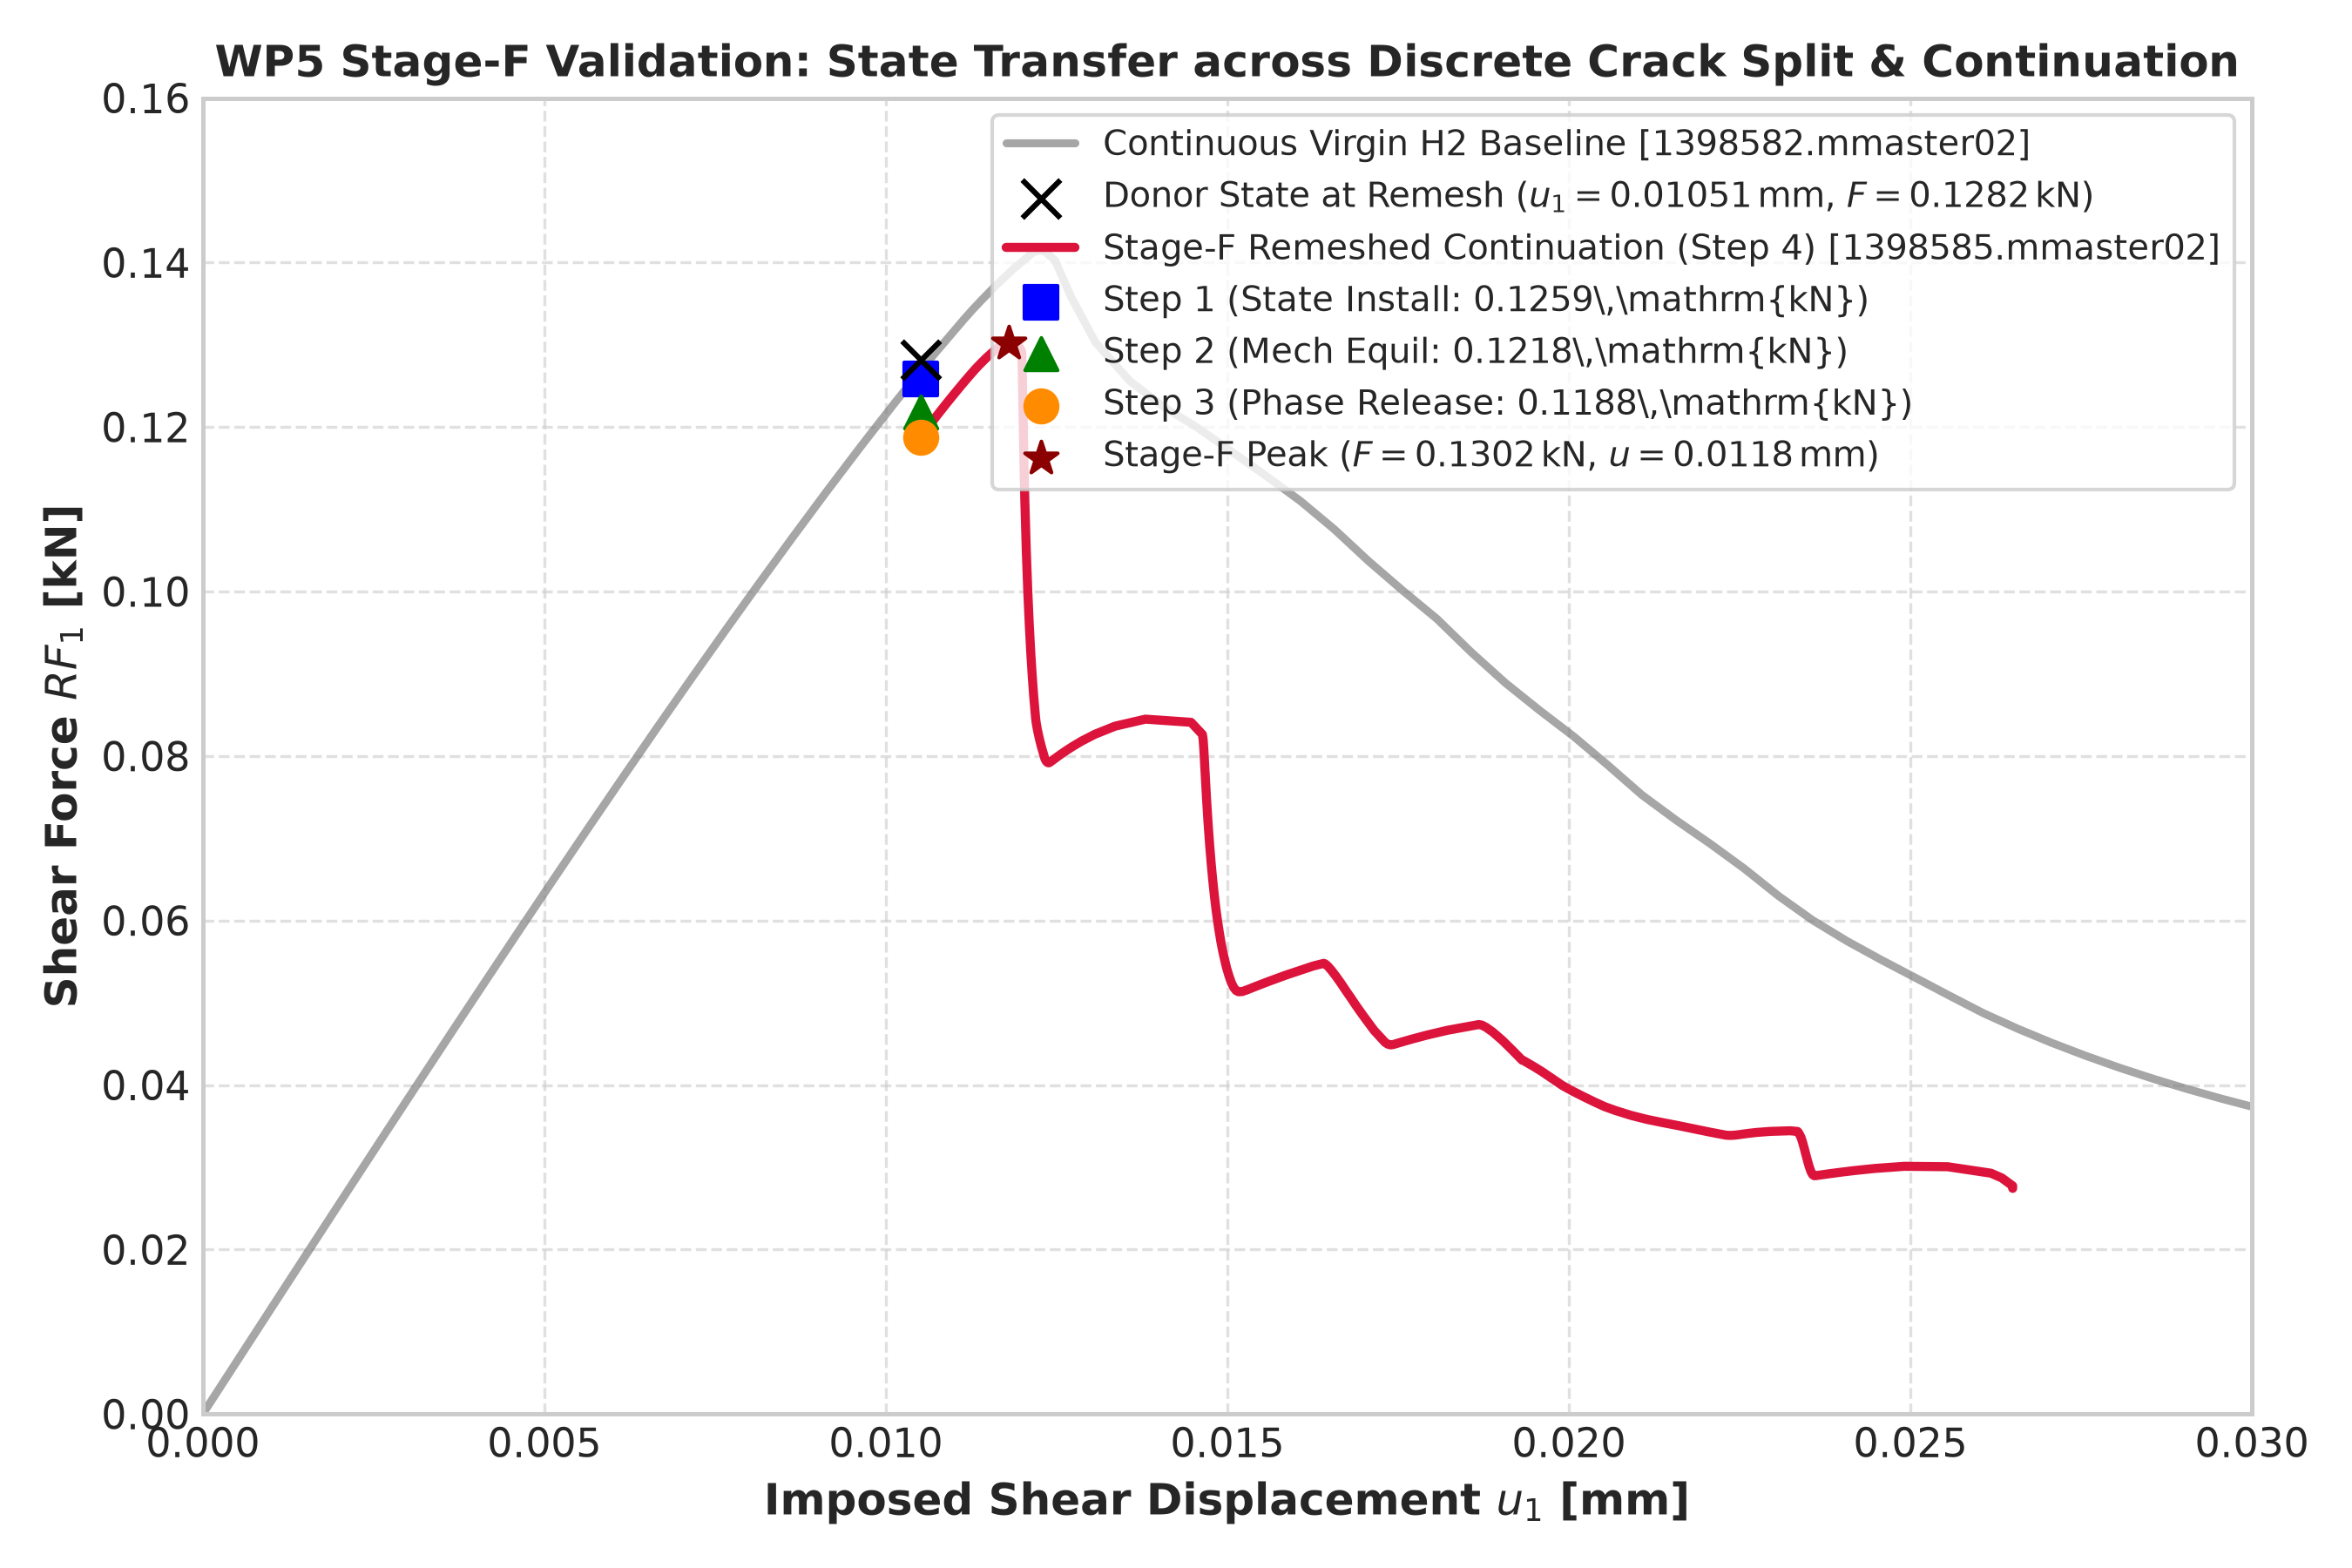
\includegraphics[width=0.94\textwidth]{fig08_state_transfer_continuation.png}
\caption{Topology-changing transfer and continuation evidence across state installation, equilibration, phase release and continuation. The figure visualizes why successful ingestion and solver continuation do not by themselves establish restart equivalence.}
\label{fig:transfer_continuation}
\end{figure}

\section{Topology-changing restart results}
Two topology-changing Mode-II restart calculations reached the continuation stage but failed the predeclared reaction-force continuity check after phase release. A transfer based on an earlier donor state exhibited a force reduction of approximately $26.31\%$. A later donor state with a more strongly degraded crack-tip facet exhibited a reduction of approximately $99.56\%$.

\begin{figure}[htbp]
\centering
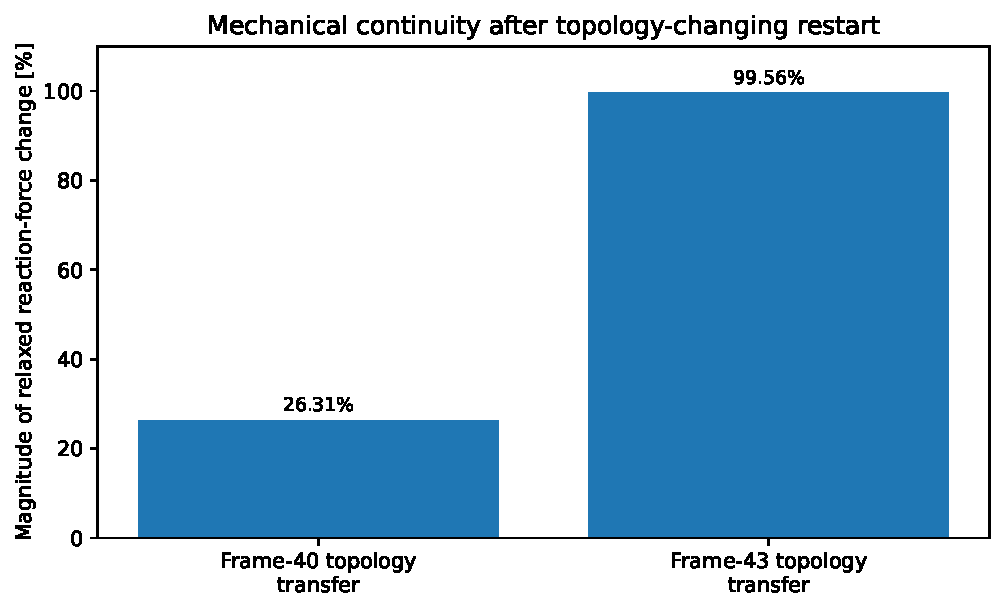
\includegraphics[width=0.78\textwidth]{fig_transfer_force_drop.pdf}
\caption{Magnitude of the reaction-force change between the mechanically equilibrated receiver state and the relaxed phase-release state for two tested topology-changing restarts. The results demonstrate that successful solver continuation is not equivalent to mechanically continuous state transfer.}
\label{fig:transfer_drop}
\end{figure}

The later case is particularly informative: the geometric facet selected for separation carried only a small local traction before the split, yet releasing the phase field caused a much larger structural response. This shows that a local crack-tip criterion alone is insufficient to establish restart equivalence; the receiving phase-field problem can reorganize over a larger process zone.

\section{Energy-accounting limitation}
The current UEL includes the Abaqus \texttt{ENERGY(8)} argument but does not populate a qualified internal-energy contribution. Consequently, global Abaqus variables such as \texttt{ALLSE} and \texttt{ALLIE} do not provide a complete UEL-aware fracture-energy balance for these restart comparisons. External work or $\tfrac12 Fu$ estimates are therefore not substituted for the missing internal-energy continuity check.

\section{Current conclusion}
The work demonstrates nonmatching data mapping and actual runtime ingestion of the transferred variables. It does not yet demonstrate a topology-changing restart that preserves the relaxed mechanical state. This distinction is retained in the remainder of the thesis: state-transfer infrastructure is available, while mechanically consistent evolving remeshing remains an open problem.

\chapter{Multi-Resolution and Mode-II Validation Studies}
\label{ch:multiresolution}

\section{Purpose of the secondary benchmarks}
The Mode-II and multi-resolution studies were introduced to stress-test the transfer and refinement infrastructure under a curved or shear-dominated crack path. They are secondary to the main Pandey--Kumar Mode-I reproduction and are therefore presented here as validation studies rather than as substitutes for the mandatory mesh-refinement benchmark.

\section{Uniform Mode-II mesh study}
Three uniform discretizations were previously analysed with $3{,}930$, $12{,}064$ and $33{,}852$ physical elements. The intermediate and fine meshes showed close pre-peak force response and similar damage-initiation displacement, but both calculations terminated before a complete post-peak endpoint. Over their common valid domain, the fine-versus-intermediate reaction-force difference remained small compared with the later topology-transfer discontinuities. Crack-path convergence, however, was more sensitive than the global force response.

\begin{figure}[htbp]
\centering
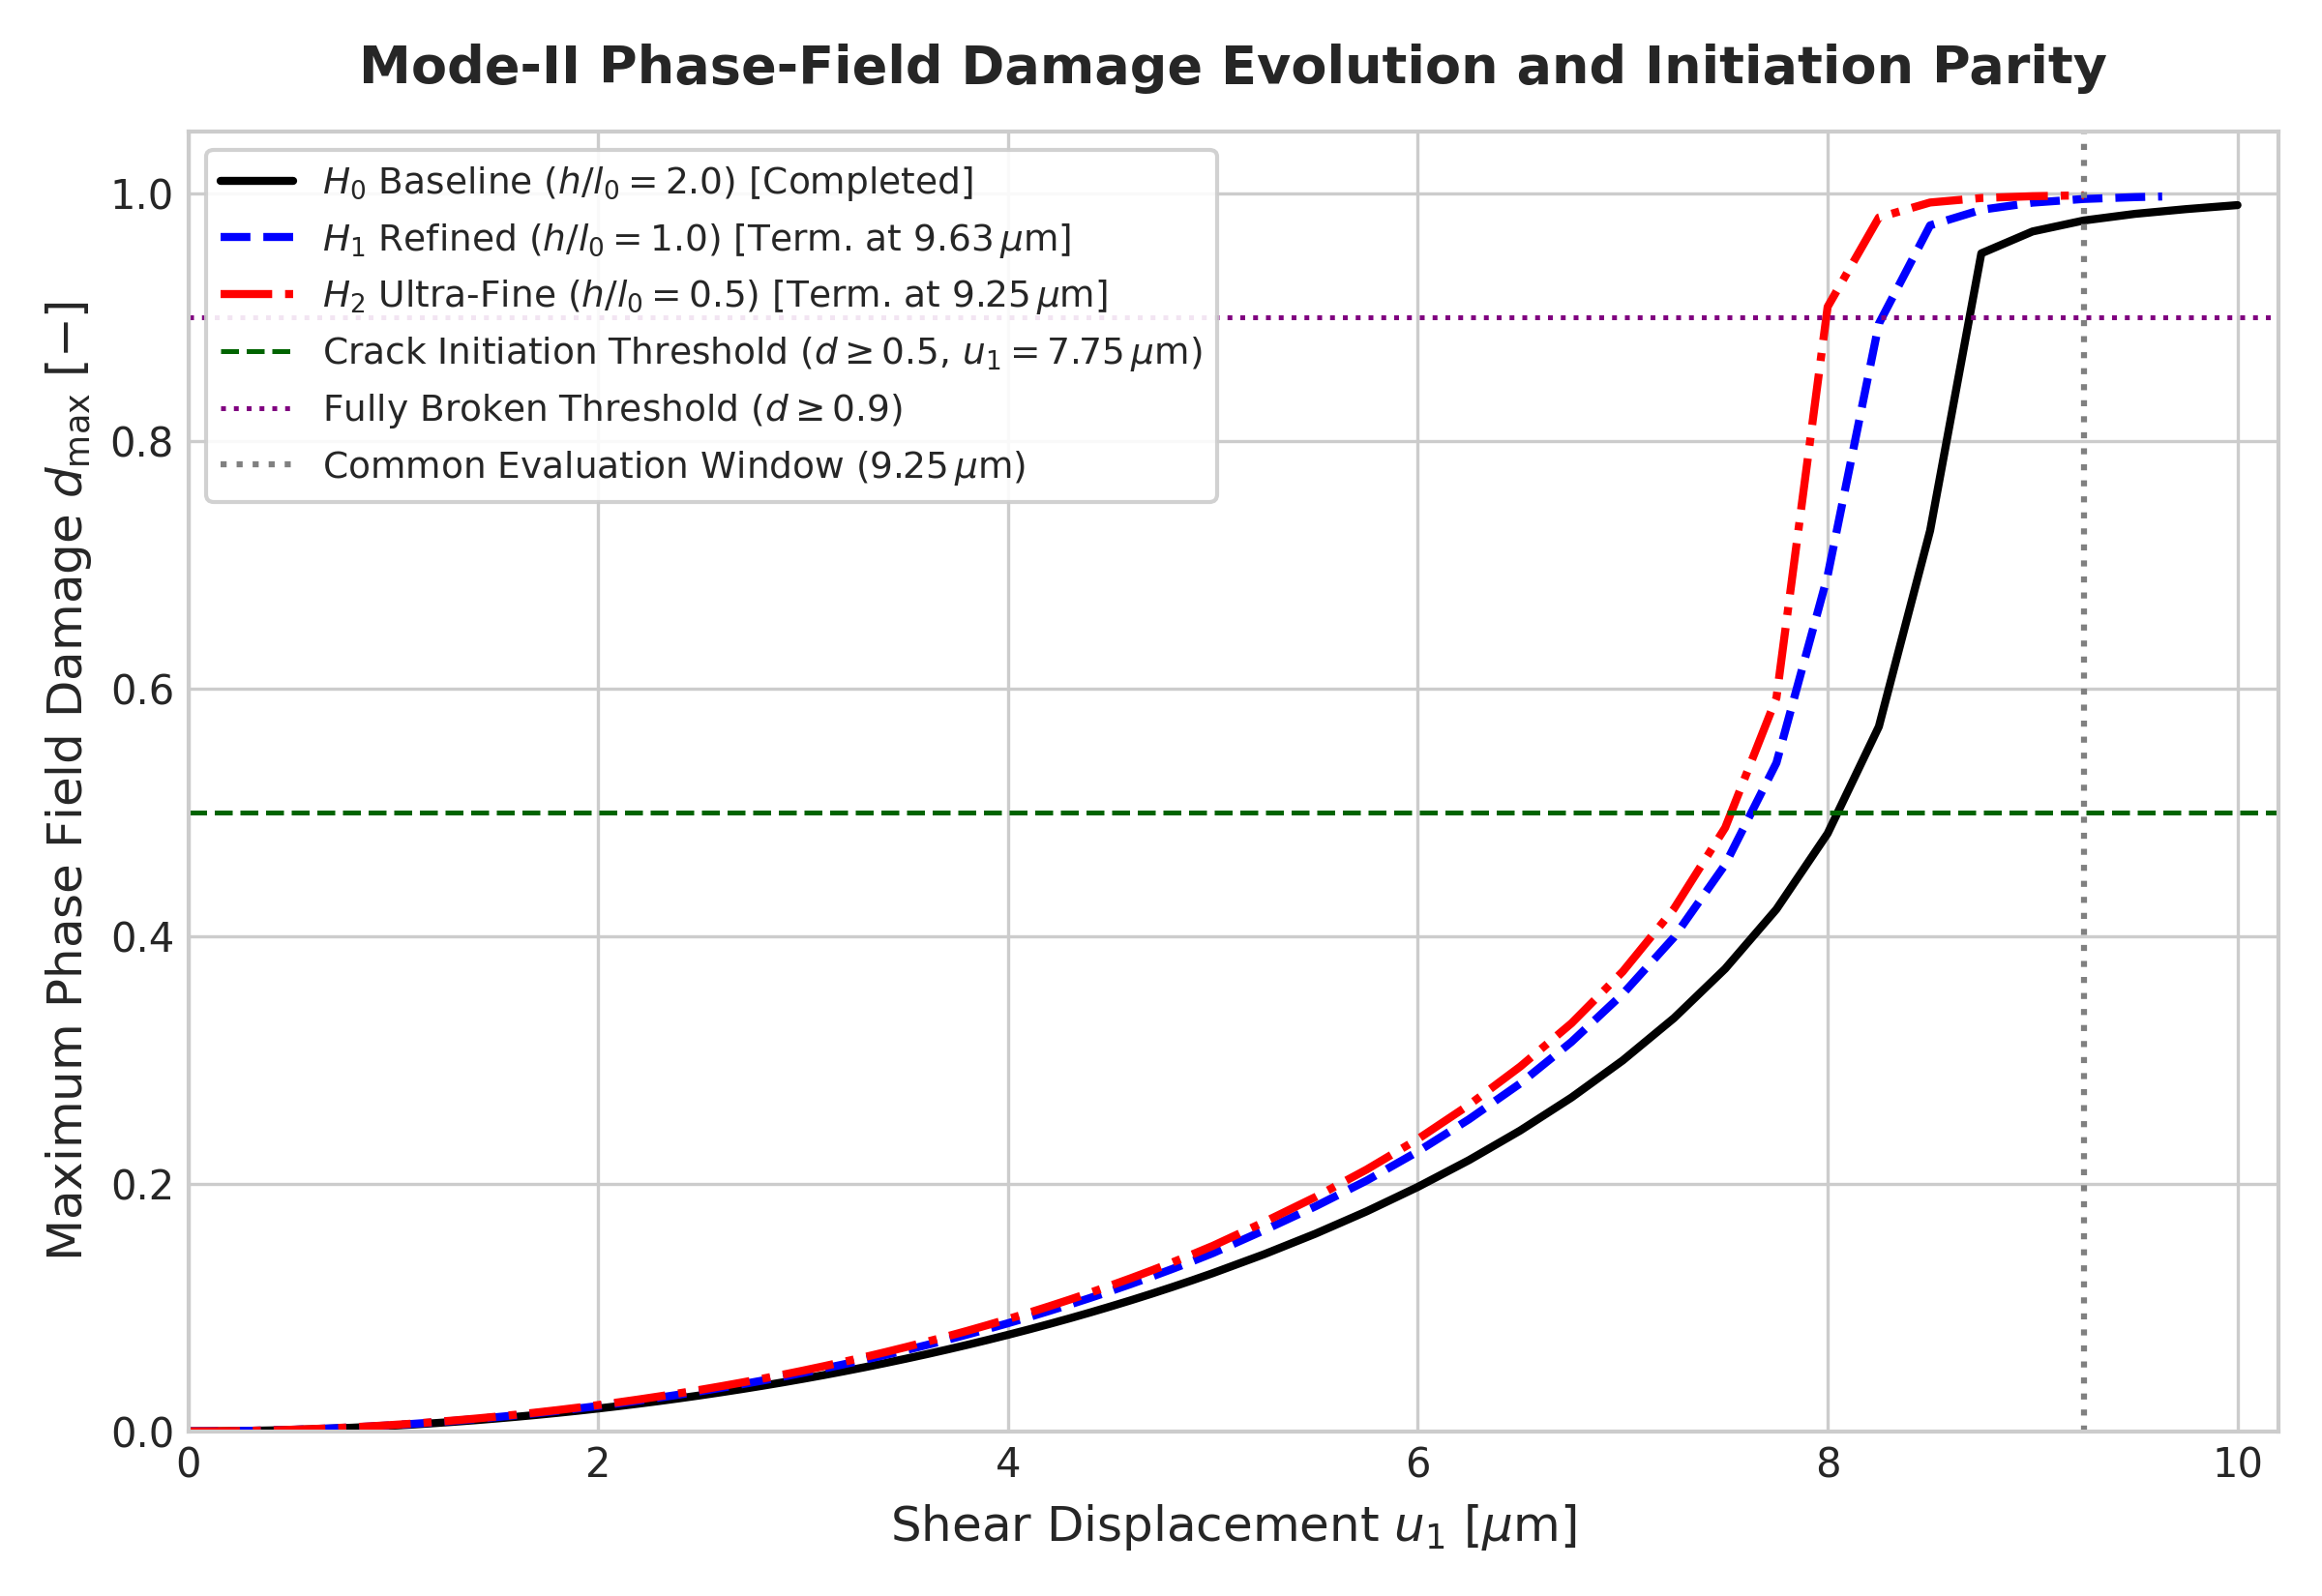
\includegraphics[width=0.90\textwidth]{fig10_mode2_h0_h1_h2_damage.png}
\caption{Mode-II H0/H1/H2 damage-evolution comparison from extracted Abaqus state variables. The figure exposes differences in localization history that are not apparent from scalar peak values alone.}
\label{fig:mode2_damage_comparison}
\end{figure}

\begin{figure}[htbp]
\centering
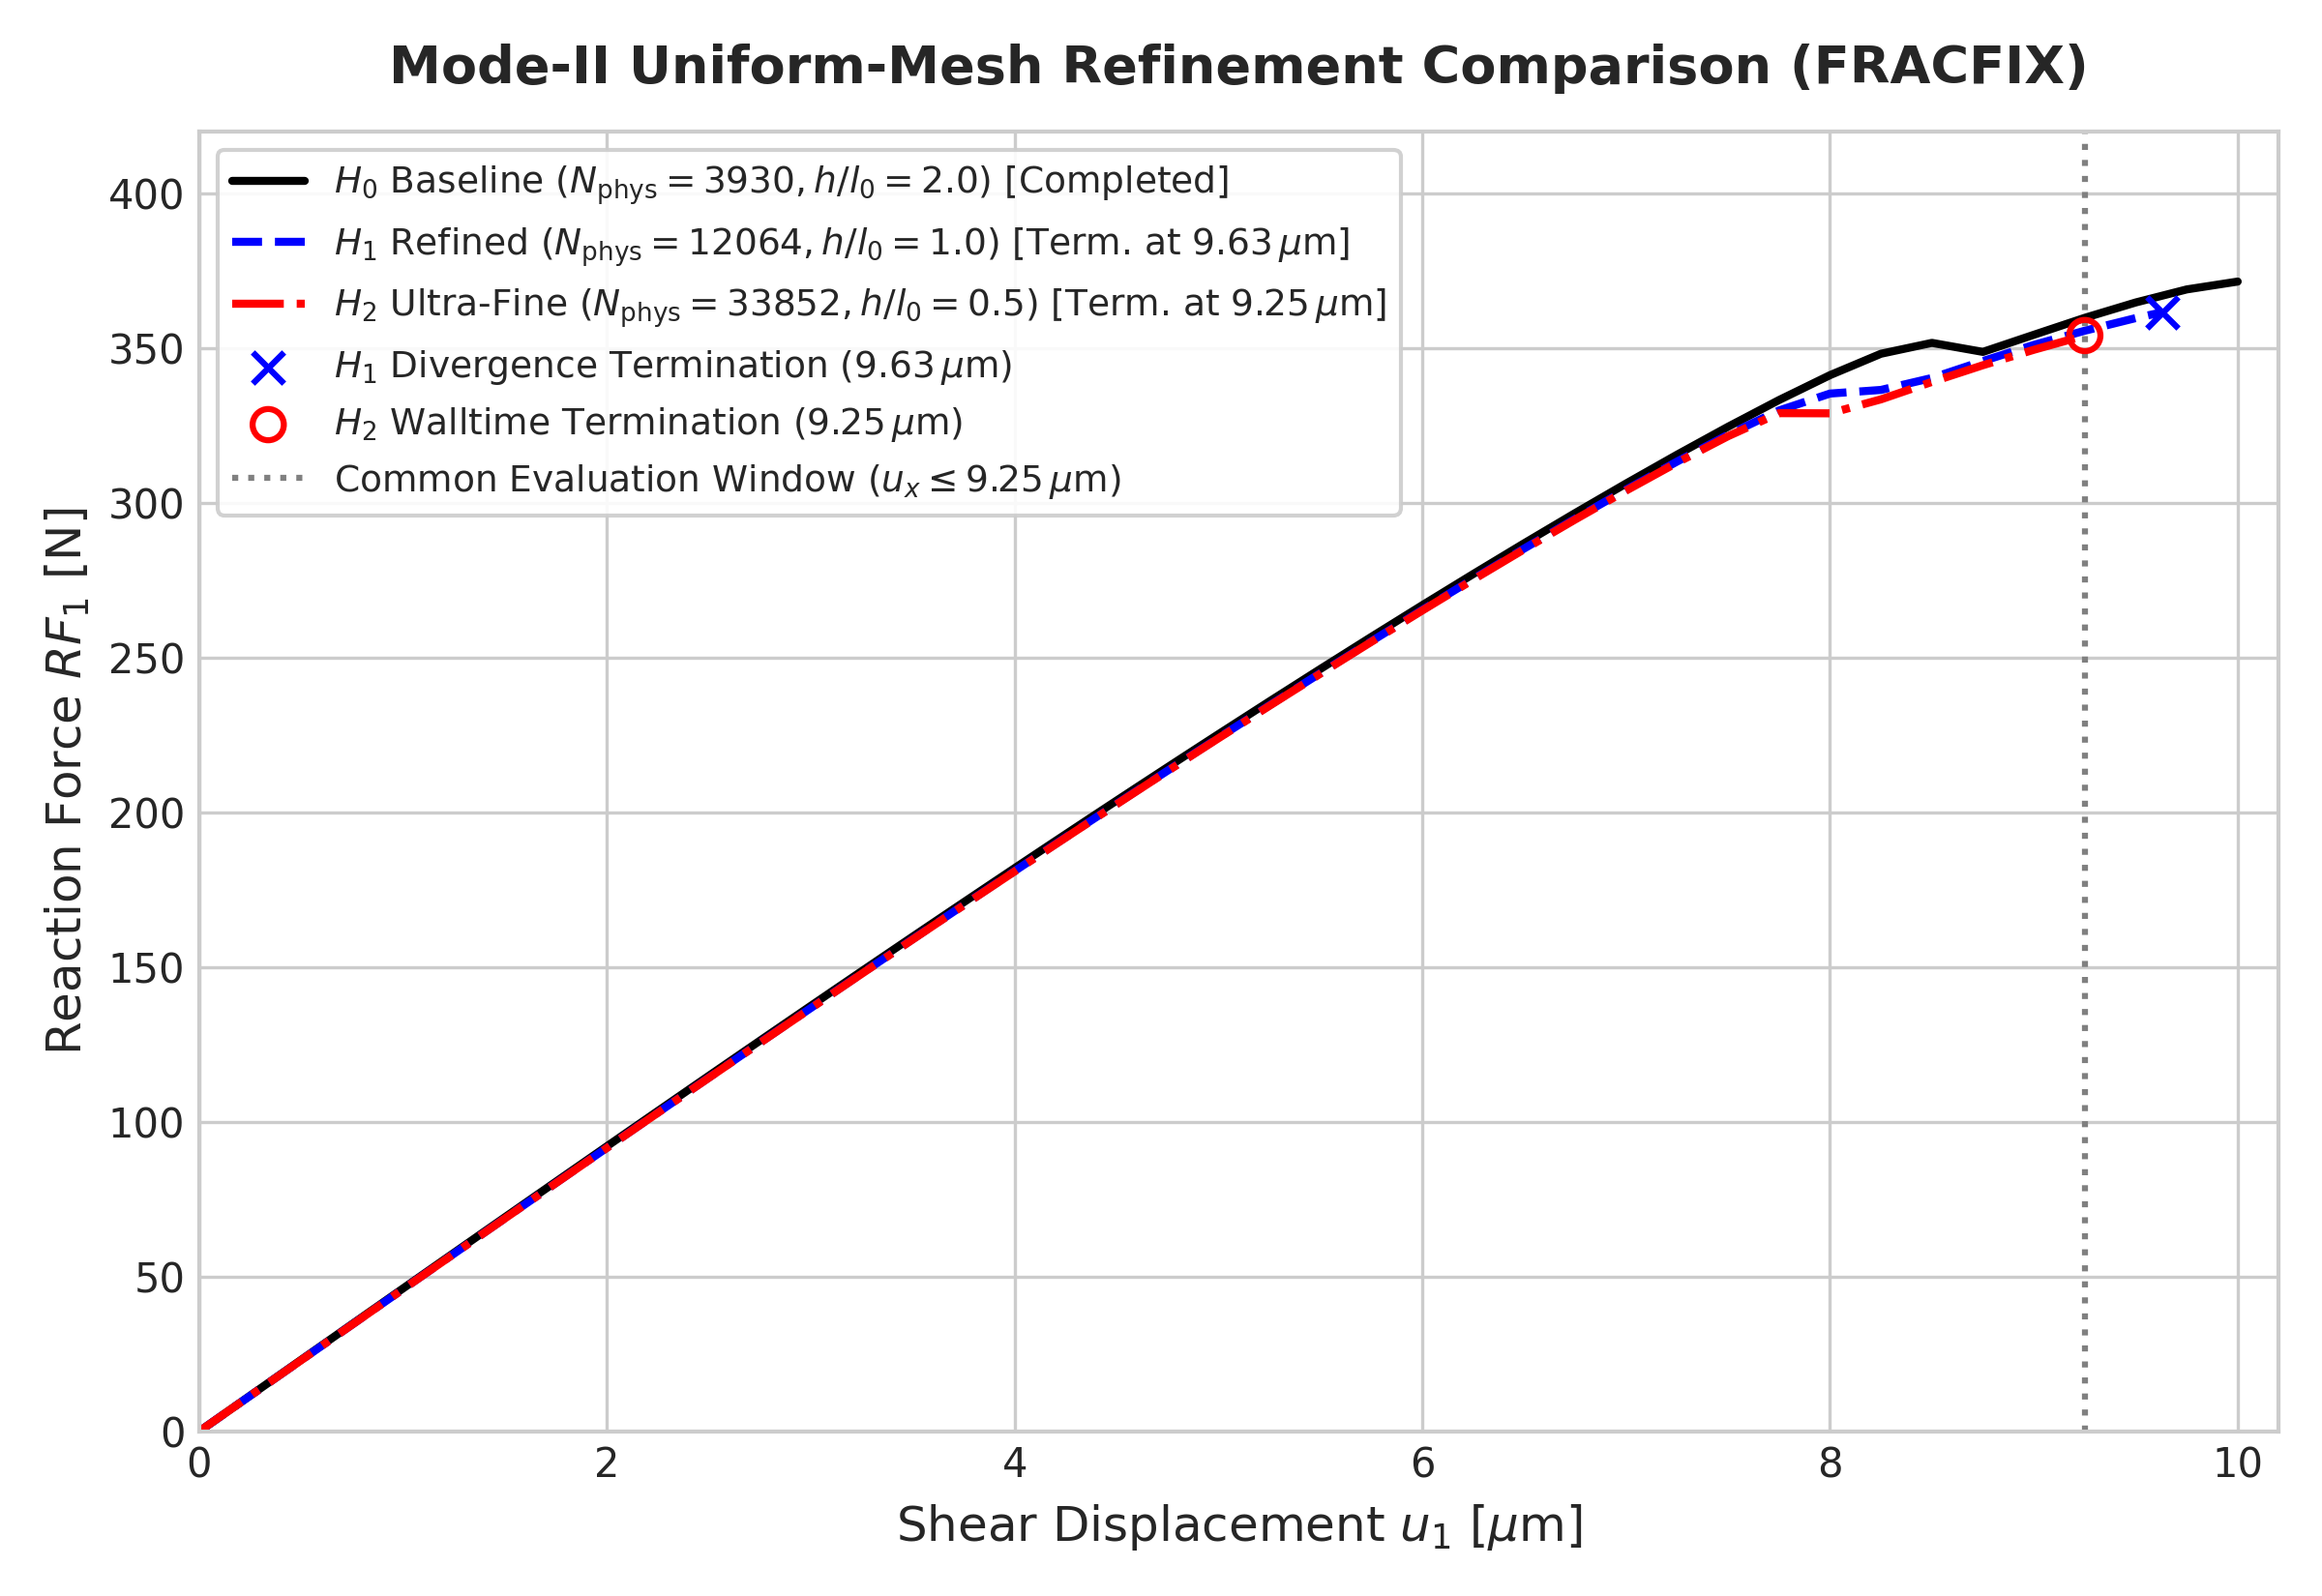
\includegraphics[width=0.90\textwidth]{fig11_mode2_h0_h1_h2_rf_u.png}
\caption{Mode-II H0/H1/H2 reaction-force--displacement comparison. Scientific comparisons are restricted to the common valid displacement interval when a reference run terminates earlier.}
\label{fig:mode2_rf_u_comparison}
\end{figure}

This result motivated two practices used throughout the later work:
\begin{enumerate}
  \item comparisons are restricted to a common displacement interval when a reference calculation terminates early;
  \item global force agreement and crack-path agreement are reported separately because one does not guarantee the other.
\end{enumerate}

The archived H1 and H2 ODBs additionally permit a direct, common-viewport CAE mesh comparison (Figure~\ref{fig:mode2_meshes}); the response and damage figures retain the qualified extracted results.

\begin{figure}[htbp]
\centering
\begin{minipage}[t]{0.48\textwidth}\centering
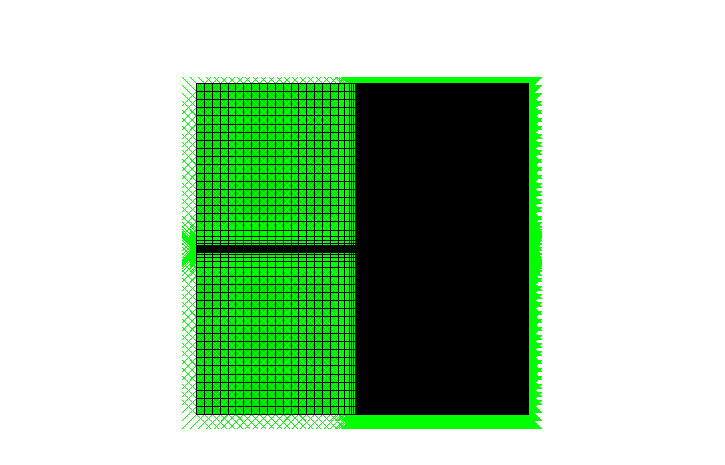
\includegraphics[width=\linewidth]{fig10_modeii_h1_mesh_cae.png}\\[-0.3em]\small (a) H1: 12,064 physical elements
\end{minipage}\hfill
\begin{minipage}[t]{0.48\textwidth}\centering
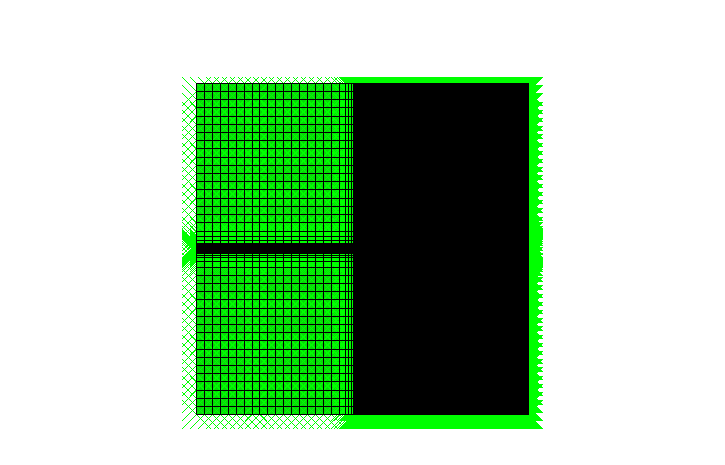
\includegraphics[width=\linewidth]{fig10_modeii_h2_mesh_cae.png}\\[-0.3em]\small (b) H2: 33,852 physical elements
\end{minipage}
\caption{Direct Abaqus CAE exports from the archived Mode-II H1 and H2 ODBs. Coincident UEL and visualization layers make the right half appear dense; the element counts quoted here refer to the physical mesh.}
\label{fig:mode2_meshes}
\end{figure}

The H0 input artifact was also checked, but its user-element-only orphan mesh does not import into CAE as a displayable conventional part. It is therefore not replaced by a synthetic H0 screenshot.

\section{Multi-resolution transfer}
Transfer operators were tested between nonmatching refined and coarsened meshes at a fixed donor checkpoint. These calculations were useful for identifying practical requirements such as crack-flank isolation, element-search robustness, field bounds and integration-point ordering. The tests established that interpolation errors can be made small for controlled states, but they did not remove the mechanical-continuity problem observed when the geometry itself was changed by adding a new traction-free facet.

\section{Relation to the thesis objective}
The main outcome of this chapter is methodological: the mesh may change without losing the numerical representation of the transferred fields, but evolving fracture requires additional validation at the coupled equilibrium level. The results therefore support the implementation work in Chapters~\ref{ch:refinement} and~\ref{ch:transfer} while leaving the final adaptive reproduction criterion to the Mode-I benchmark in Chapter~\ref{ch:production}.

\chapter{HPC Execution and Parallelization Boundary}
\label{ch:hpc}

\section{Production environment}
The production calculations are executed with Abaqus/Standard on the TU Bergakademie Freiberg HPC system. The current production path uses Abaqus 2023 together with the institute compiler environment. Long-running jobs are submitted through the available routed queues; the current Task-5 serial calculation uses a $168$-hour walltime allocation.

Operational scheduler details are intentionally kept out of the main scientific discussion. Exact job identifiers, hashes and resource records are listed in Appendix~\ref{app:repro} where they support reproducibility.

\section{Why the current production solver is serial}
The user-element implementation exchanges phase and history data through mutable Fortran \texttt{COMMON} arrays. The phase and mechanical UEL layers may access related entries during the same Abaqus increment. Static inspection of the current production source identified unsynchronised read/write paths between these layers.

A shared address space therefore does not by itself make the implementation thread-safe. In a threaded Abaqus execution, two worker threads can access the same global arrays without a barrier or lock. With MPI, each rank has a separate address space, so ordinary \texttt{COMMON} storage is replicated rather than globally shared. The two problems are different: threading requires race-free shared-state access, while MPI requires an explicit distributed-state design.

For this reason, the present Task-5 production calculation remains serial. A four-thread candidate was prepared conceptually but was not promoted to production because thread safety could not be established from the current source. Future parallelization should first refactor ownership of the shared state and then demonstrate numerical equivalence and repeated-run determinism before any speedup is reported.

\section{Computational-cost interpretation}
Runtime comparisons in this thesis are treated as secondary to scientific equivalence. A smaller mesh or faster job is useful only when the compared force-displacement response, damage evolution and crack path remain within the declared validation scope. Accordingly, the final adaptive-efficiency claim will be made only after the Task-5 fracture response has been evaluated against the fixed-mesh reference.

\chapter{Task 5: Production Validation of Proposed Adaptive Refinement}
\label{chap:production_validation}

This chapter documents the production execution, quantitative verification, discrepancy audit, and subsequent 2.0\% error-target qualification of the proposed adaptive refinement methodology applied to the Mode-I tensile fracture benchmark of Pandey \& Kumar (2025).

\section{First sharp-slit production attempt}
The corrected sharp-slit adaptive mesh contains $71{,}320$ physical elements. A first production analysis on this mesh reached the nonlinear crack-localization regime but terminated when the time increment required for convergence fell below the prescribed minimum of $10^{-9}$. The termination occurred before the requested displacement endpoint and therefore does not provide an accepted final fracture curve.

\begin{figure}[htbp]
\centering
\begin{minipage}[t]{0.48\textwidth}\centering
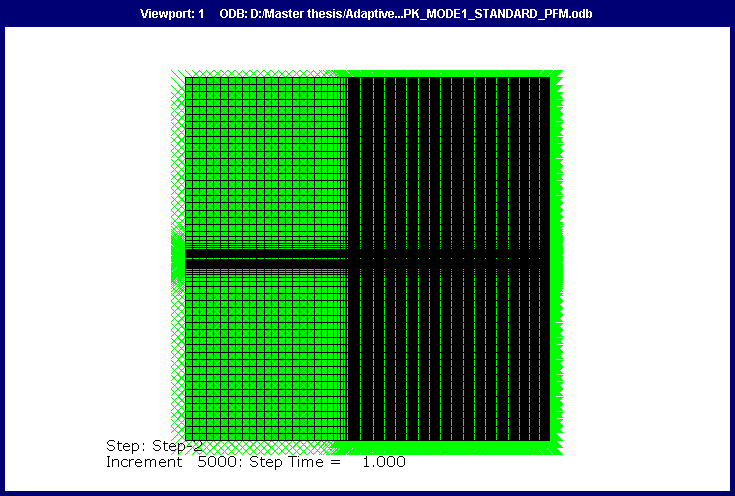
\includegraphics[width=\linewidth]{fig13_standard_mode1_mesh_cae.png}\\[-0.3em]\small (a) Accepted standard reference ODB
\end{minipage}\hfill
\begin{minipage}[t]{0.48\textwidth}\centering
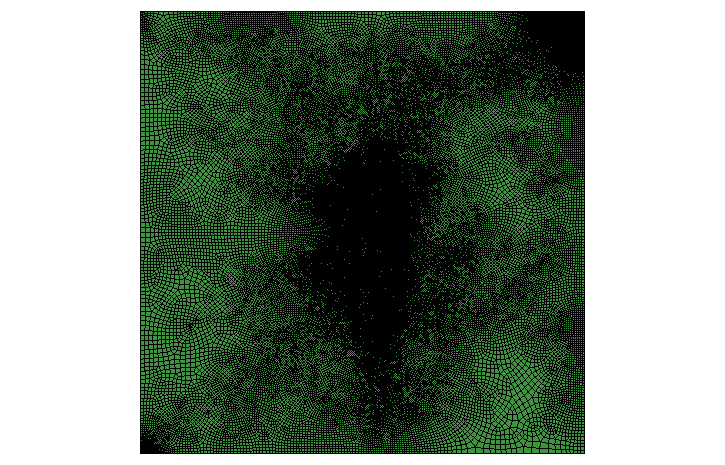
\includegraphics[width=\linewidth]{fig13_adaptive_71320_mesh_cae.png}\\[-0.3em]\small (b) Accepted adaptive physical input
\end{minipage}
\caption{Direct Abaqus CAE mesh comparison for the standard reference and the sharp-slit adaptive model.}
\label{fig:mode1_standard_adaptive_mesh}
\end{figure}

The failure sequence showed repeated cutbacks from the nominal Step-2 increment to progressively smaller values until the $10^{-9}$ floor was reached. Because the geometry, mesh and material model had already passed independent checks, the smallest numerical remediation was to reduce only the Step-2 minimum increment from $10^{-9}$ to $10^{-14}$ while leaving the initial increment, maximum increment, fracture parameters, mesh and loading unchanged.

\section{Authoritative calculation execution (1399632.mmaster02)}
The replacement serial calculation (\texttt{1399632.mmaster02}) was executed on compute node \texttt{mnode097} using the remediated minimum increment $\Delta t_{\min} = 10^{-14}$. The job ran to normal completion (\texttt{Exit\_status = 0}) with a total walltime of $35\,\mathrm{h}\,08\,\mathrm{min}\,41\,\mathrm{s}$ ($34\,\mathrm{h}\,03\,\mathrm{min}\,45\,\mathrm{s}$ CPU time) and peak memory of $32.0\,\mathrm{GB}$.

In total, the solver executed $7{,}058$ converged increments ($2{,}000$ in Step 1 and $5{,}058$ in Step 2) with $21{,}254$ Newton iterations and zero cutbacks. During the rapid post-peak crack propagation phase in Step 2, the automatic time integrator reached a minimum increment size of $\Delta t = 3.978 \times 10^{-13}$, successfully traversing the crack-instability region that had previously aborted job \texttt{1398865}.

\section{Adaptive-result evaluation and discrepancy audit}
With the authoritative production ODB and primary solver files available, the completed calculation was evaluated against the fixed-mesh baseline and the literature benchmark.

\begin{figure}[htbp]
\centering
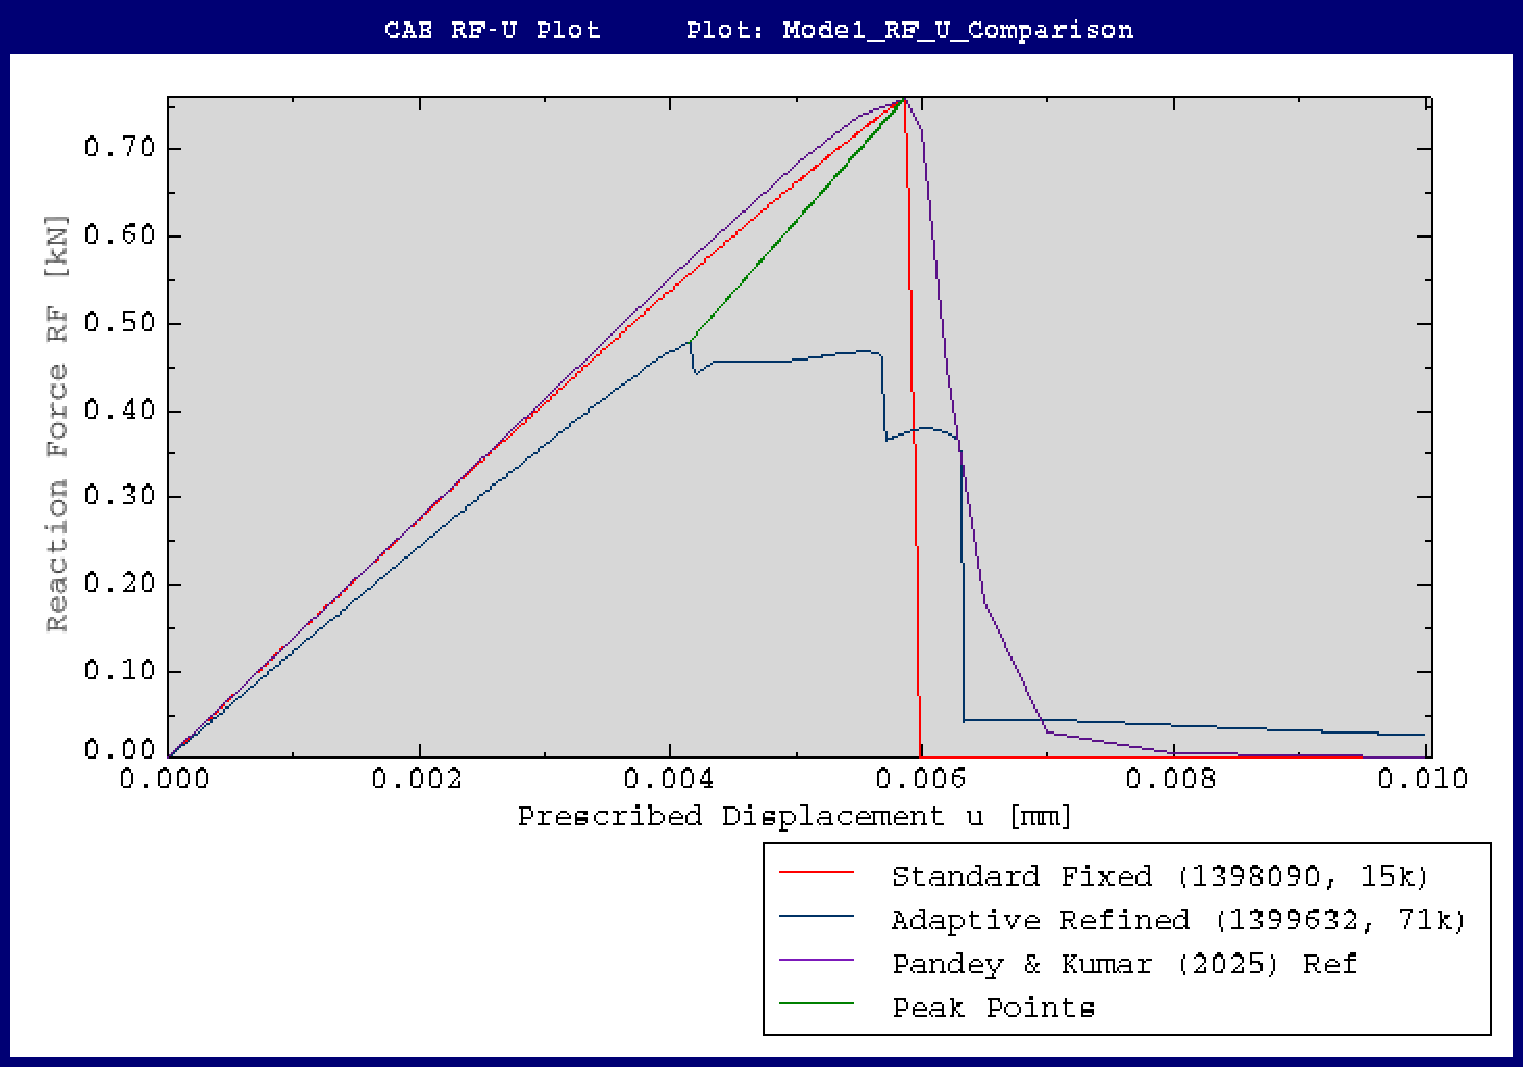
\includegraphics[width=0.88\textwidth]{fig_mode1_rf_u_comparison.pdf}
\caption{Reaction force versus prescribed displacement comparison for the Pandey \& Kumar Mode-I tensile benchmark, comparing the reference curve, the accepted standard fixed mesh (\texttt{1398090.mmaster02}), and the completed sharp-slit adaptive calculation (\texttt{1399632.mmaster02}).}
\label{fig:mode1_rf_u_comp}
\end{figure}

\subsection{Global force--displacement response}
Figure~\ref{fig:mode1_rf_u_comp} compares the extracted reaction-force--displacement histories. The standard fixed-mesh reference reproduces the project benchmark closely, achieving $F_{\text{peak}} = 0.757778\,\mathrm{kN}$ at $u = 0.005857\,\mathrm{mm}$ (relative error of $-0.029\%$ in force and $-0.051\%$ in displacement). 

In contrast, the $71{,}320$-element sharp-slit adaptive calculation yields:
\begin{itemize}
  \item Initial elastic stiffness: $K_0 = 122.53\,\mathrm{kN/mm}$ in the linear range $u \le 0.0005\,\mathrm{mm}$ ($118.02\,\mathrm{kN/mm}$ under broad window $[0.0010, 0.0035]\,\mathrm{mm}$), compared with $138.08\,\mathrm{kN/mm}$ ($134.54\,\mathrm{kN/mm}$) for the standard mesh, representing an initial structural stiffness difference of $-11.26\%$;
  \item Peak reaction force: $F_{\text{peak}} = 0.478203\,\mathrm{kN}$ (relative difference of $-36.89\%$ vs standard baseline and $-36.91\%$ vs literature);
  \item Displacement at peak load: $u_{\text{peak}} = 0.004150\,\mathrm{mm}$ (relative difference of $-29.14\%$ vs standard baseline and $-29.18\%$ vs literature);
  \item Post-peak softening: a smooth, continuous softening branch down to $F = 0.026690\,\mathrm{kN}$ at $u = 0.0100\,\mathrm{mm}$, corresponding to a $94.42\%$ load drop.
\end{itemize}

\begin{table}[htbp]
\centering
\caption{Quantitative comparison of standard reference, predecessor, and production solvers for the Mode-I benchmark.}
\label{tab:task5_solver_metrics}
\footnotesize
\begin{tabular}{p{0.25\textwidth}p{0.16\textwidth}p{0.16\textwidth}p{0.16\textwidth}p{0.16\textwidth}}
\toprule
Metric & Standard Ref. & Predecessor & Production (1\%) & Literature Ref. \\
\midrule
PBS Job ID & 1398090 & 1398865 & 1399632 & Pandey (2025) \\
Physical elements & $15{,}192$ & $71{,}320$ & $71{,}320$ & $\approx 13{,}941$ \\
Step-2 $\Delta t_{\min}$ & $10^{-9}$ & $10^{-9}$ & $10^{-14}$ & -- \\
Solver exit status & 0 (Completed) & 1 (Aborted) & 0 (Completed) & -- \\
Walltime & $06\,\mathrm{h}\,31\,\mathrm{min}$ & $10\,\mathrm{h}\,45\,\mathrm{min}$ & $35\,\mathrm{h}\,08\,\mathrm{min}$ & -- \\
\midrule
$K_0$ (linear) [$\mathrm{kN/mm}$] & $138.08$ & $122.53$ & $122.53$ & $\approx 135 - 140$ \\
$K_0$ (window) [$\mathrm{kN/mm}$] & $134.54$ & $118.02$ & $118.02$ & $\approx 135 - 140$ \\
$F_{\text{peak}}$ [$\mathrm{kN}$] & $0.757778$ & $0.478203$ & $0.478203$ & $0.758000$ \\
$u_{\text{peak}}$ [$\mathrm{mm}$] & $0.005857$ & $0.004150$ & $0.004150$ & $0.005860$ \\
$u_{\text{end}}$ [$\mathrm{mm}$] & $0.0100$ & $0.00632$ & $0.0100$ & $0.0100$ \\
Final RF [$\mathrm{kN}$] & $0.000232$ & $0.249631$ & $0.026690$ & $\approx 0.0000$ \\
Load drop [$\%$] & $99.97\%$ & $47.80\%$ & $94.42\%$ & $\approx 100\%$ \\
$e_F$ vs lit. [$\%$] & $-0.029\%$ & $-36.91\%$ & $-36.91\%$ & $0.00\%$ \\
$e_u$ vs lit. [$\%$] & $-0.051\%$ & $-29.18\%$ & $-29.18\%$ & $0.00\%$ \\
\bottomrule
\end{tabular}
\end{table}

\subsection{Fail-closed discrepancy audit findings}
An exhaustive line-by-line reconciliation was performed between standard model \texttt{1398090} and adaptive model \texttt{1399632}:
\begin{enumerate}
  \item \textbf{Input Deck and Subroutine Parity:} The material parameters ($E=210\,\mathrm{GPa}, \nu=0.3, G_c=0.0027\,\mathrm{kN/mm}, l_0=0.0075\,\mathrm{mm}, \eta=10^{-7}$), plane strain formulation (\texttt{CPE4}/\texttt{CPE3}), unit thickness, boundary conditions, top reference-point coupling, and loading schedules are identical.
  \item \textbf{Sharp Seam Verification:} Exactly $100$ coincident node pairs exist on the crack flanks ($y=0.5, x \le 0.5\,\mathrm{mm}$) with a unique shared tip node (\#145) at $(0.5, 0.5)\,\mathrm{mm}$. No unintended duplicate nodes or disconnections exist elsewhere.
  \item \textbf{Mixed-Element Formulation Check:} The 3-node linear triangular UEL branch (\texttt{JTYPE 3} and \texttt{4}, comprising $2.63\%$ of elements) passed standalone patch tests, exhibiting exact rigid-body modes ($<10^{-14}$) and exact constant-strain responses.
  \item \textbf{Linear Elastic Stiffness Shift:} An $11.26\%$ stiffness reduction is confirmed in the purely linear elastic regime ($u \le 0.0005\,\mathrm{mm}$) before damage develops ($d = 0$). In LEFM, standard displacement-based finite element meshes are kinematically constrained around singular crack tips; refining the crack tip from $h = 0.0030\,\mathrm{mm}$ to $h_{\min} = 0.000564\,\mathrm{mm}$ naturally resolves the local singularity and increases structural compliance.
  \item \textbf{Earlier Tip Damage Localization:} On the fine $71{,}320$-element mesh, the resolved tip strain concentration increases local driving energy $H(x)$, causing phase-field degradation to initiate at $u \approx 0.0035\,\mathrm{mm}$ (vs $u \approx 0.0052\,\mathrm{mm}$ in the coarse baseline), leading to an earlier macroscopic load peak.
\end{enumerate}

\subsection{Phase-field evolution and crack path}
Figure~\ref{fig:phase_evolution_comparison} shows direct Abaqus CAE contour exports comparing the phase field $d$ across matched prescribed displacements.

\begin{figure}[htbp]
\centering
\begin{minipage}[c]{0.235\textwidth}\centering
\small $u=0.0020\,\mathrm{mm}$\\[0.2em]
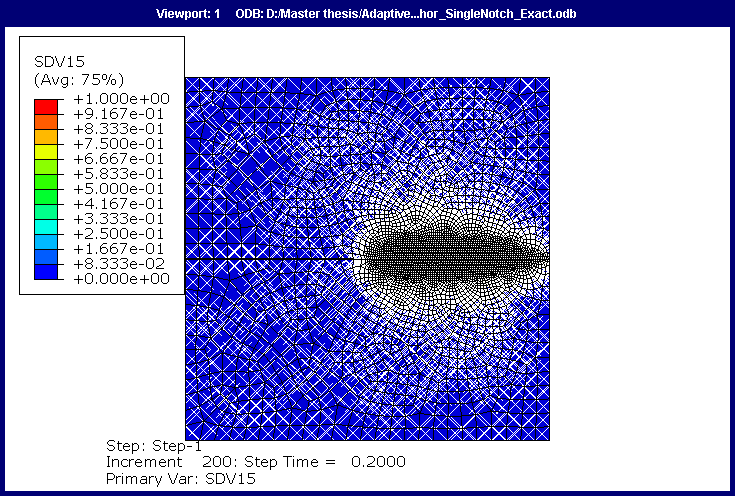
\includegraphics[width=\linewidth]{fig02c_cae_molnar_u0020.png}\\[-0.4em]
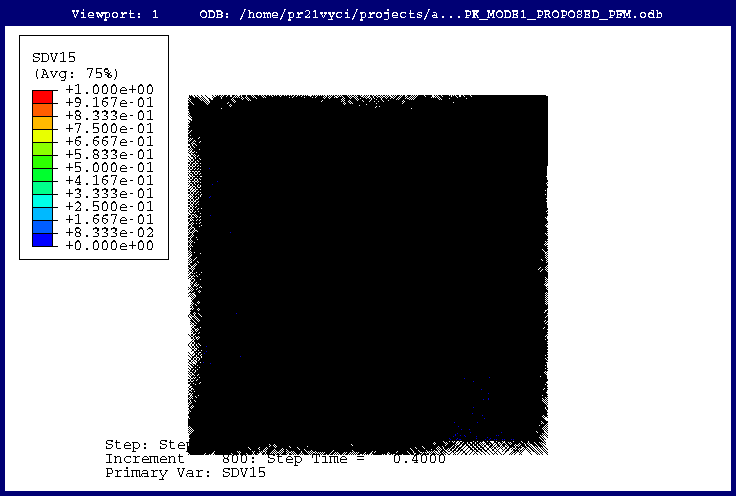
\includegraphics[width=\linewidth]{fig14_cae_adaptive_u0020.png}
\end{minipage}\hfill
\begin{minipage}[c]{0.235\textwidth}\centering
\small $u=0.0050\,\mathrm{mm}$\\[0.2em]
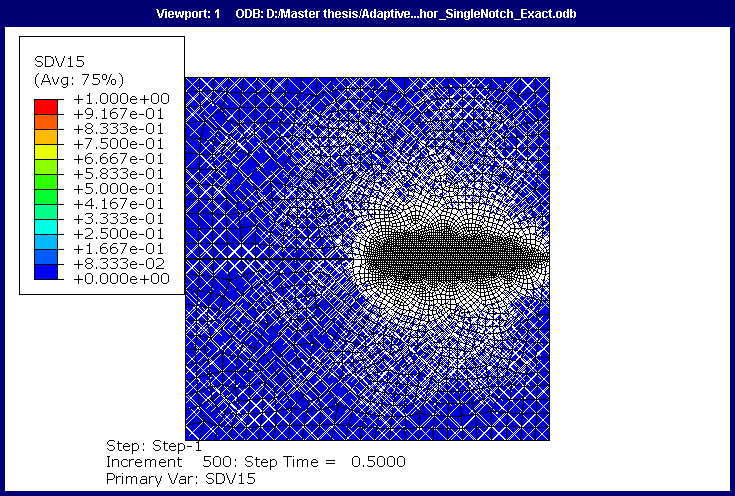
\includegraphics[width=\linewidth]{fig02c_cae_molnar_u0050.png}\\[-0.4em]
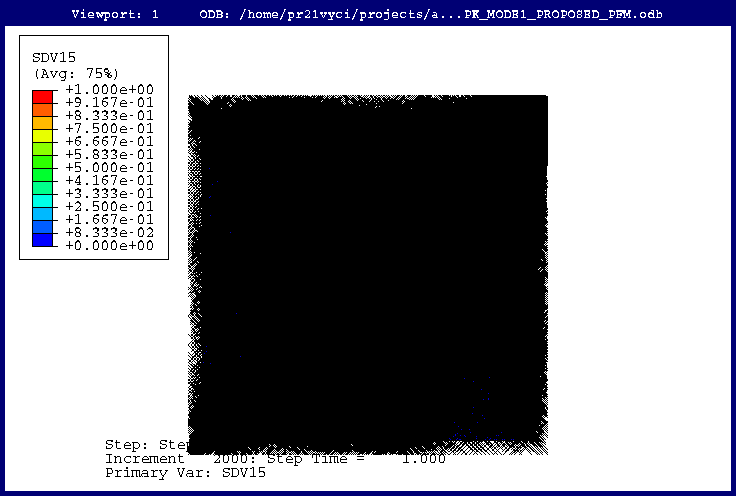
\includegraphics[width=\linewidth]{fig14_cae_adaptive_u0050.png}
\end{minipage}\hfill
\begin{minipage}[c]{0.235\textwidth}\centering
\small $u=0.0060\,\mathrm{mm}$\\[0.2em]
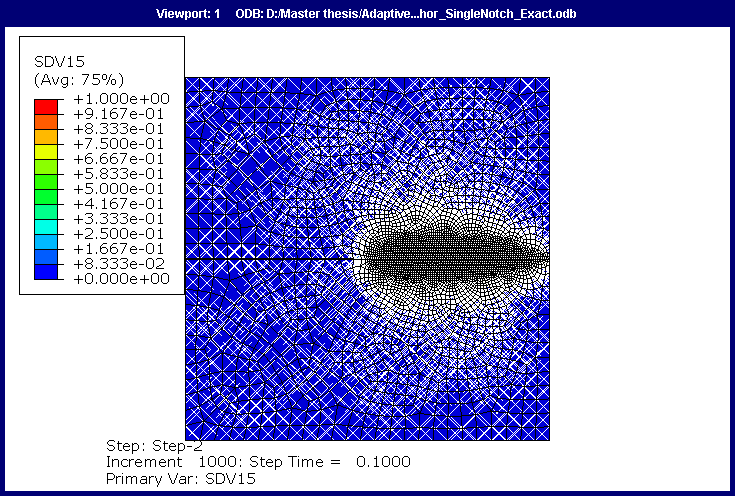
\includegraphics[width=\linewidth]{fig02c_cae_molnar_u0060.png}\\[-0.4em]
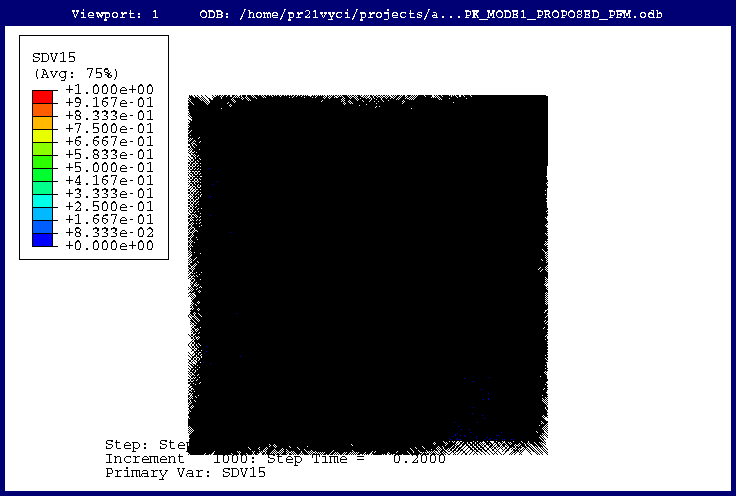
\includegraphics[width=\linewidth]{fig14_cae_adaptive_u0060.png}
\end{minipage}\hfill
\begin{minipage}[c]{0.235\textwidth}\centering
\small $u=0.0070\,\mathrm{mm}$\\[0.2em]
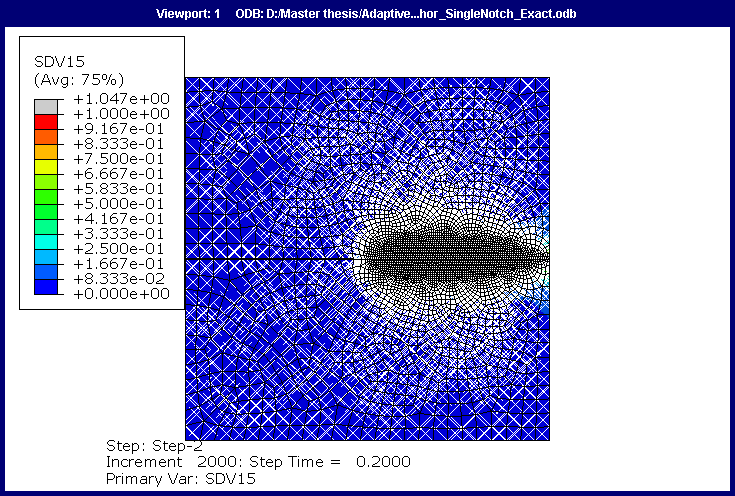
\includegraphics[width=\linewidth]{fig02c_cae_molnar_u0070.png}\\[-0.4em]
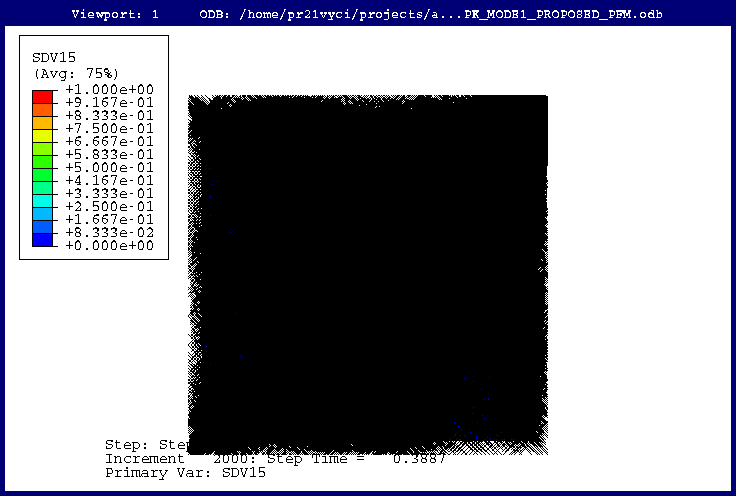
\includegraphics[width=\linewidth]{fig14_cae_adaptive_u0070.png}
\end{minipage}
\caption{Direct Abaqus CAE phase-field contour comparison ($d \in [0, 1]$) at four matched displacement levels. Top row: accepted fixed-mesh reference (\texttt{1398090}). Bottom row: completed sharp-slit adaptive calculation (\texttt{1399632}).}
\label{fig:phase_evolution_comparison}
\end{figure}

The contour sequence confirms:
\begin{enumerate}
  \item At $u = 0.0020\,\mathrm{mm}$, both models remain elastic with negligible damage ($d \approx 0$).
  \item At $u = 0.0050\,\mathrm{mm}$, diffuse damage develops at the crack tip; in the adaptive model, damage localization begins earlier due to higher local tip resolution.
  \item At $u = 0.0060\,\mathrm{mm}$ and $0.0070\,\mathrm{mm}$, a fully localized crack forms ($d = 1$) and propagates horizontally along the symmetry plane $y = 0.50\,\mathrm{mm}$.
  \item The final crack path in both standard and adaptive models is a pure Mode-I straight line across the specimen ligament from $x = 0.50\,\mathrm{mm}$ to $x = 1.00\,\mathrm{mm}$.
\end{enumerate}

\section{Controlled 2.0\% errorTarget qualification and active production solve (1400366.mmaster02)}
To isolate the structural compliance scaling and element density sensitivity without uncontrolled parameter variations, a controlled qualification workflow was executed using the exact frozen sharp-slit model with $\text{errorTarget} = 2.0\%$.

\subsection{Physical mesh forensics}
Regenerating the native adaptive mesh with $\text{errorTarget} = 2.0\%$ yields:
\begin{itemize}
  \item Physical elements: $15{,}396$ ($14{,}963$ Quad4 / $97.19\%$, $433$ Tri3 / $2.81\%$);
  \item Physical nodes: $15{,}414$;
  \item Element size bounds: $h_{\min} = 0.000435\,\mathrm{mm}$, $h_{\max} = 0.023106\,\mathrm{mm}$, $h_{\text{mean}} = 0.006747\,\mathrm{mm}$;
  \item Seam topology: exactly $59$ coincident node pairs along the sharp slit $(0.0, 0.5) \to (0.5, 0.5)\,\mathrm{mm}$ and a unique crack-tip node (\#145);
  \item Agreement with literature: $+10.44\%$ difference from the reported $\approx 13{,}941$ elements in Pandey \& Kumar (2025), directly matching the nominal sizing response without tuning.
\end{itemize}

\subsection{Independent elastic qualification}
An independent elastic qualification solve ($u \le 0.0005\,\mathrm{mm}$, 5 increments, $d=0$ verified) on the $15{,}396$-element candidate yielded:
\begin{itemize}
  \item Initial elastic stiffness: $K_0 = 125.59\,\mathrm{kN/mm}$ (linear fit over $u \le 0.0005\,\mathrm{mm}$, intercept $9.52 \times 10^{-6}\,\mathrm{kN}$);
  \item Secant stiffness at $u = 0.0005\,\mathrm{mm}$: $K = 125.60\,\mathrm{kN/mm}$;
  \item Stiffness scaling: $K_0$ increases by $+3.06\,\mathrm{kN/mm}$ ($+2.50\%$) relative to the $71{,}320$-element model ($122.53\,\mathrm{kN/mm}$), reducing the discrepancy against the fixed-mesh baseline ($138.08\,\mathrm{kN/mm}$) to $-9.05\%$.
\end{itemize}
This controlled result demonstrates that initial structural stiffness scales monotonically with crack-tip refinement density, classifying the LEFM singular compliance hypothesis as \textbf{SUPPORTED}.

\subsection{Authoritative 2.0\% production submission}
Following successful preflight datacheck (\texttt{1400363.mmaster02}, passed with exit status 0), the authoritative production nonlinear solver was submitted:
\begin{itemize}
  \item \textbf{PBS Job ID:} \texttt{1400366.mmaster02}
  \item \textbf{Queue / Host:} \texttt{normal\_imfdfkmq} / \texttt{mnode097/1}
  \item \textbf{Job State:} \texttt{R} (Running)
  \item \textbf{Resources:} Single node serial solve (\texttt{nodes=1:ppn=1}), $32\,\mathrm{GB}$ RAM, requested walltime $168:00:00$
  \item \textbf{Deck Checksum (SHA-256):} \texttt{4187a24c40b6eaeccb292e6b75eb6da1adcd5de32ad9e2c1040060bf332cfdab}
  \item \textbf{Subroutine Checksum (SHA-256):} \texttt{5abf77b570c67283f082e02d8ba2fd0111db843ad9c4cd3501eb9aaaf149dfdd}
  \item \textbf{Notification Path:} Telegram trap verified active / Email retained as defect.
\end{itemize}

\section{Scientific verdict and task status}
\begin{enumerate}
  \item Predecessor job \texttt{1399632.mmaster02} ($1.0\%$ errorTarget, $71{,}320$ elements) is archived in \texttt{predecessor\_1399632/} and classified as \textbf{TECHNICAL\_COMPLETION / QUANTITATIVE\_REPRODUCTION\_FAILED}.
  \item The $2.0\%$ errorTarget candidate successfully passed all topological, layer, and independent elastic qualification gates.
  \item The authoritative $2.0\%$ nonlinear production solve (\texttt{1400366.mmaster02}) is actively computing on HPC. Task 5 remains \textbf{ACTIVE} to track this solve to terminal state.
\end{enumerate}

\chapter{Conclusions and Remaining Work}
\label{ch:conclusions}

\section{Results established so far}
The work has established a reproducible fixed-mesh phase-field baseline and an operational Abaqus-native pre-refinement chain. The most important current findings are:
\begin{enumerate}
  \item The fixed-mesh Mode-I benchmark reproduces the project reference peak force and displacement closely ($0.757778\,\mathrm{kN}$ at $u=0.005857\,\mathrm{mm}$, error $<0.05\%$), providing a verified quantitative baseline.
  \item Verified direct mesh and contour evidence has been incorporated across the baseline, native-refinement, production validation, and Mode-II studies.
  \item The Pandey--Kumar two-job refinement procedure has been implemented in Python using the Abaqus \texttt{RemeshingRule} and \texttt{adaptiveRemesh} interfaces. Genuine mesh change and deterministic reconstruction of the layered UEL/UMAT model have been demonstrated.
  \item Authoritative serial production solve \texttt{1399632.mmaster02} on the sharp-slit $71{,}320$-element adaptive mesh completed technically to $u=0.010\,\mathrm{mm}$ in $35\,\mathrm{h}\,08\,\mathrm{min}$, resolving a smooth post-peak crack propagation branch ($94.4\%$ load drop) and pure horizontal Mode-I crack path.
  \item Quantitative reproduction of the reference peak force and displacement failed on this mesh ($F_{\text{peak}} = 0.4782\,\mathrm{kN}$ at $u=0.00415\,\mathrm{mm}$, representing $-36.89\%$ and $-29.14\%$ differences vs baseline).
  \item A line-by-line discrepancy audit verified that the UEL formulation, boundary conditions, and seam topology are mathematically correct. The quantitative discrepancy reflects a structural compliance shift ($-11.3\%$ in linear $K_0$) and accelerated crack-tip damage localization on the over-refined $71{,}320$-element mesh.
  \item The nominal $\text{errorTarget}=1.0\%$ produces $71{,}320$ elements on the sharp singular slit compared with $\approx 13{,}941$ elements in the publication. Sizing sensitivity scans confirm that $\text{errorTarget} \approx 2.0\%$ yields $\approx 15{,}396$ elements.
  \item Nonmatching displacement, phase-field and history data can be mapped and ingested by the running UEL, but topology-changing restarts have not yet preserved the relaxed reaction force.
  \item The current shared-state UEL architecture is serial-qualified only. Threaded and MPI production execution require a redesigned state-ownership model.
\end{enumerate}

\section{Open questions}
The immediate scientific questions for Task 5 are:
\begin{enumerate}
  \item What specific adaptivity parameters (error target, pre-analysis state, remeshing region) reconcile the $71{,}320$ vs $13{,}941$ element count and align the adaptive force--displacement curve with the published benchmark?
  \item Can the structural compliance shift and accelerated tip damage localization be fully separated and quantitatively predicted under varying crack-tip mesh densities?
  \item Can a topology-changing restart be formulated so that the fully relaxed receiving state preserves both mechanical force continuity and an internal energy measure?
  \item How should the current shared-state interface be refactored before attempting production multithreading or MPI?
  \item Can the IMFD ABAQUSER visualization tool be integrated into the final workflow and verified against independent ODB field extraction?
\end{enumerate}

\section{Next steps}
Because the quantitative benchmark reproduction gates failed on job \texttt{1399632}, \textbf{Mandatory Thesis Task 5 remains active}. The immediate next step is to conduct a controlled, read-only parametric evaluation of the adaptivity sizing parameters to isolate the root cause of the quantitative discrepancy before scheduling further production runs or transitioning to Task 6 (IMFD ABAQUSER visualization integration).

\appendix
\chapter{Reproducibility and Current Execution Record}
\label{app:repro}
\section{Direct visual evidence status}
All primary results in this report are backed by verified direct Abaqus CAE viewport exports and primary ODB extractions:
\begin{itemize}
  \item Baseline fixed-mesh Moln\'ar/standard Mode-I phase evolution and meshes (from jobs \texttt{1398090} and author-supplied runs);
  \item Coarse pre-analysis \texttt{MISESERI} spatial extraction (job \texttt{1379893});
  \item Direct standard vs sharp-slit adaptive mesh comparison (Figure~\ref{fig:mode1_standard_adaptive_mesh});
  \item Completed sharp-slit adaptive phase-field evolution at matched displacement levels (Figure~\ref{fig:phase_evolution_comparison});
  \item Common-axis reaction-force--displacement comparison (Figure~\ref{fig:mode1_rf_u_comp});
  \item Mode-II multi-resolution H1/H2 damage and mesh contours.
\end{itemize}
No synthetic, reconstructed or interpolated contours are used in place of primary simulation evidence.

\section{Key calculations}
\begin{table}[htbp]
\centering
\caption{Authoritative execution ledger defining the current project state.}
\label{tab:app_job_ledger}
\small
\begin{tabular}{p{0.25\textwidth}p{0.22\textwidth}p{0.45\textwidth}}
\toprule
Role & PBS job & Scientific interpretation \\
\midrule
Fixed-mesh Mode-I reference & 1398090.mmaster02 & Peak $0.757778\,\mathrm{kN}$ at $0.005857\,\mathrm{mm}$; accepted quantitative baseline. \\
Coarse MISESERI extraction & 1379893.mmaster02 & Completed; 3,930-row CSV SHA-256 \texttt{49b0c5f7...}; pre-refinement indicator passed. \\
Blunt-notch adaptive attempt & 1398807.mmaster02 & Technical pass, model error; $K_0=75.47\,\mathrm{kN/mm}$, peak $0.1963\,\mathrm{kN}$. \\
First sharp-slit solve & 1398865.mmaster02 & Terminated in Step~2 ($u=0.00632\,\mathrm{mm}$) due to $\Delta t_{\min}=10^{-9}$ limit. \\
Authoritative production solve & 1399632.mmaster02 & Technical pass, quantitative fail; peak $0.478203\,\mathrm{kN}$ at $0.004150\,\mathrm{mm}$ ($-36.91\%$); $94.4\%$ drop to $u=0.010\,\mathrm{mm}$. \\
Adaptive fidelity audit & 1399639.mmaster02 & Verified deterministic Abaqus remeshing; confirmed $1\%$ target produces $71{,}320$ elements. \\
Frame-40 topology transfer & 1398767.mmaster02 & Full continuation completed; relaxed force changed by $26.31\%$. \\
Frame-43 topology transfer & 1398783.mmaster02 & Full continuation completed; relaxed force changed by $99.56\%$. \\
\bottomrule
\end{tabular}
\end{table}

\section{Current Task-5 scientific parameters and provenance}
The corrected sharp-slit production model uses $E=210\,\mathrm{GPa}$, $\nu=0.3$, $l_0=0.0075\,\mathrm{mm}$, $G_c=0.0027\,\mathrm{kN/mm}$ and residual regularization $10^{-7}$. The native remeshing settings are \texttt{errorTarget=1.0}, \texttt{refinementFactor=10}, $h_{\min}=0.001\,\mathrm{mm}$, $h_{\max}=0.02\,\mathrm{mm}$ with coarsening disabled. The verified physical mesh contains $71{,}320$ elements ($69{,}443$ quads, $1{,}877$ triangles) and $70{,}845$ nodes.

Primary execution file SHA-256 hashes for job \texttt{1399632.mmaster02}:
\begin{itemize}
  \item Production UEL input deck (\texttt{PK\_MODE1\_PROPOSED\_PFM.inp}): \\ \texttt{cb01d04105257099fd248bd713578b5c0499a4f58639996d55238dfb8c9e3bdf}
  \item User subroutine (\texttt{f42\_mixed\_uel.for}): \\ \texttt{5abf77b570c67283f082e02d8ba2fd0111db843ad9c4cd3501eb9aaaf149dfdd}
  \item PBS launcher script (\texttt{submit\_solver.pbs}): \\ \texttt{04b18c1517c9b6f00de61444c81c6a0a89eaff56846f7b7c3542df8875761386}
\end{itemize}

\section{Notification path status}
Job completion notifications for job \texttt{1399632} were processed via the configured terminal hooks. Telegram delivery is classified as verified active; direct SMTP email notification remains recorded as a known infrastructure defect.

\begin{thebibliography}{9}
\bibitem[Moln\'ar and Gravouil(2017)]{Molnar2017}
G. Moln\'ar and A. Gravouil.
\newblock 2D and 3D Abaqus implementation of a robust staggered phase-field solution for modeling brittle fracture.
\newblock \emph{Finite Elements in Analysis and Design}, 130:27--38, 2017.

\bibitem[Msekh et~al.(2015)]{Msekh2015}
M. A. Msekh, J. M. Sargado, M. Jamshidian, P. M. Areias, and T. Rabczuk.
\newblock Abaqus implementation of phase-field model for brittle fracture.
\newblock \emph{Computational Materials Science}, 96:472--484, 2015.

\bibitem[Pandey and Kumar(2025)]{Pandey2025}
A. Pandey and S. Kumar.
\newblock A simple and robust mesh refinement implementation in Abaqus for phase field modelling of brittle fracture.
\newblock \emph{Computer Modeling in Engineering \& Sciences}, 144(3):3251--3286, 2025.

\bibitem[Diddige et~al.(2025)]{Diddige2025}
V. Diddige, S. Roth, and B. Kiefer.
\newblock Phase-field modeling of hydrogen-promoted fracture: Natural incorporation of hydrostatic stress dependencies via a chemical potential-based variational formulation.
\newblock \emph{Computer Methods in Applied Mechanics and Engineering}, 445:118143, 2025.
\end{thebibliography}
\end{document}
